%%
%% This is file `sample-sigconf.tex',
%% generated with the docstrip utility.
%%
%% The original source files were:
%%
%% samples.dtx  (with options: `sigconf')
%% 
%% IMPORTANT NOTICE:
%% 
%% For the copyright see the source file.
%% 
%% Any modified versions of this file must be renamed
%% with new filenames distinct from sample-sigconf.tex.
%% 
%% For distribution of the original source see the terms
%% for copying and modification in the file samples.dtx.
%% 
%% This generated file may be distributed as long as the
%% original source files, as listed above, are part of the
%% same distribution. (The sources need not necessarily be
%% in the same archive or directory.)
%%
%% Commands for TeXCount
%TC:macro \cite [option:text,text]
%TC:macro \citep [option:text,text]
%TC:macro \citet [option:text,text]
%TC:envir table 0 1
%TC:envir table* 0 1
%TC:envir tabular [ignore] word
%TC:envir displaymath 0 word
%TC:envir math 0 word
%TC:envir comment 0 0
%%
%%
%% The first command in your LaTeX source must be the \documentclass command.
\documentclass[sigconf]{acmart}
%% NOTE that a single column version is required for 
%% submission and peer review. This can be done by changing
%% the \doucmentclass[...]{acmart} in this template to 
%% \documentclass[manuscript,screen]{acmart}
%% 
%% To ensure 100% compatibility, please check the white list of
%% approved LaTeX packages to be used with the Master Article Template at
%% https://www.acm.org/publications/taps/whitelist-of-latex-packages 
%% before creating your document. The white list page provides 
%% information on how to submit additional LaTeX packages for 
%% review and adoption.
%% Fonts used in the template cannot be substituted; margin 
%% adjustments are not allowed.

%%
%% \BibTeX command to typeset BibTeX logo in the docs
\AtBeginDocument{%
  \providecommand\BibTeX{{%
    \normalfont B\kern-0.5em{\scshape i\kern-0.25em b}\kern-0.8em\TeX}}}

%% Rights management information.  This information is sent to you
%% when you complete the rights form.  These commands have SAMPLE
%% values in them; it is your responsibility as an author to replace
%% the commands and values with those provided to you when you
%% complete the rights form.
\setcopyright{acmlicensed}
\copyrightyear{2024}
\acmYear{2024}
\acmDOI{XXXXXXX.XXXXXXX}

%% These commands are for a PROCEEDINGS abstract or paper.
% \acmConference[MM'24]{Make sure to enter the correct
%   conference title from your rights confirmation email}{October 28 - November 1,
%   2024}{Melbourne, Australia.}
\acmConference[ACM MM]{}{October 28 - November 1, 2024}{Melbourne, Australia.}

%
%  Uncomment \acmBooktitle if th title of the proceedings is different
%  from ``Proceedings of ...''!
%
%\acmBooktitle{Woodstock '18: ACM Symposium on Neural Gaze Detection,
%  June 03--05, 2018, Woodstock, NY} 
\acmISBN{978-1-4503-XXXX-X/18/06}

\usepackage{xcolor,colortbl}

%%
%% Submission ID.
%% Use this when submitting an article to a sponsored event. You'll
%% receive a unique submission ID from the organizers
%% of the event, and this ID should be used as the parameter to this command.
%%\acmSubmissionID{123-A56-BU3}

%%
%% For managing citations, it is recommended to use bibliography
%% files in BibTeX format.
%%
%% You can then either use BibTeX with the ACM-Reference-Format style,
%% or BibLaTeX with the acmnumeric or acmauthoryear sytles, that include
%% support for advanced citation of software artefact from the
%% biblatex-software package, also separately available on CTAN.
%%
%% Look at the sample-*-biblatex.tex files for templates showcasing
%% the biblatex styles.
%%

%%
%% The majority of ACM publications use numbered citations and
%% references.  The command \citestyle{authoryear} switches to the
%% "author year" style.
%%
%% If you are preparing content for an event
%% sponsored by ACM SIGGRAPH, you must use the "author year" style of
%% citations and references.
%% Uncommenting
%% the next command will enable that style.
%%\citestyle{acmauthoryear}

%%
%% end of the preamble, start of the body of the document source.
\begin{document}

%%
%% The "title" command has an optional parameter,
%% allowing the author to define a "short title" to be used in page headers.
\title{
% 1) 
Enhancing Cross-Modal Contextual Congruence for Crowdfunding Success using Knowledge-infused Learning %\\
% 2) Knowledge-Driven Computation of Cross-Modality Contextual Congruence in Marketing Campaigns \\
% 3) Knowledge-Infused Learning to Improve Multimodal Contextual Congruence Across Modalities for Effective Marketing 
}
%%
%% The "author" command and its associated commands are used to define
%% the authors and their affiliations.
%% Of note is the shared affiliation of the first two authors, and the
%% "authornote" and "authornotemark" commands
%% used to denote shared contribution to the research.


% \author{Name}
% \affiliation{%
%   \institution{Institution}
%   % \streetaddress{1 Th{\o}rv{\"a}ld Circle}
%   \city{City}
%   \country{Country}}
% \email{xx@xx.xx}


% \author{Name}
% \affiliation{%
%   \institution{Institution}
%   % \streetaddress{1 Th{\o}rv{\"a}ld Circle}
%   \city{City}
%   \country{Country}}
% \email{xx@xx.xx}

% \author{Name}
% \affiliation{%
%   \institution{Institution}
%   % \streetaddress{1 Th{\o}rv{\"a}ld Circle}
%   \city{City}
%   \country{Country}}
% \email{xx@xx.xx}

\author{Anonymous Authors}

%%
%% By default, the full list of authors will be used in the page
%% headers. Often, this list is too long, and will overlap
%% other information printed in the page headers. This command allows
%% the author to define a more concise list
%% of authors' names for this purpose.
\renewcommand{\shortauthors}{author name and author name, et al.}

%%
%% The abstract is a short summary of the work to be presented in the
%% article.
\begin{abstract}
The digital landscape continually evolves with multimodality, enriching the online experience for users. Creators and marketers aim to weave subtle contextual cues from various modalities into congruent content to engage users with a harmonious message. This interplay of multimodal cues is often a crucial factor in attracting users' attention. However, this richness of multimodality presents a challenge to computational modeling, as the semantic contextual cues spanning across modalities need to be unified to capture the true holistic meaning of the multimodal content. This contextual meaning is critical in attracting user engagement as it conveys the intended message of the brand or the organization. 
% TK: whats the down side - lack of context?
%, which is limited in human-reasoned commonsense knowledge. 
In this work, we incorporate external commonsense knowledge from knowledge graphs to enhance the representation of multimodal data using large Visual Language Models (VLMs) and predict the success of multi-modal crowdfunding campaigns. Our results show that external knowledge commonsense bridges the semantic gap between text and image modalities, and the enhanced knowledge-infused representations improve the predictive performance of models for campaign success upon the baselines without knowledge. Our findings highlight the significance of contextual congruence in online multimodal content for engaging and successful crowdfunding campaigns.
% TK: I am not sure what you are trying to get across --- 
% 
% Overall, the abstract needs to be improved.
% ----
% What is the problem you are trying to solve? Is lack of context or common-sense knowledge the issue or missing? are you adding it to create effective marketing campaigns. Is use of common-sense key to integrating different modalities? Or is knowledge graphs the way to remove human beings from the loop for scalability?  

% I am trying to throw questions to have you organize and verbalize your thoughts more effectively.
\end{abstract}

% Trilok ----------------------
% The prevalence of smart devices with the ability to capture moments in multiple modalities has enabled users to experience multimodal information online.  However, large Language (LLMs) and Vision models (LVMs) despite promising results on many multimodal tasks, are still limited in capturing holistic meaning with cross-modal semantic relationships which multimodal Visual Language Models (VLM) require for contextual congruence.  Without explicit, common sense knowledge (e.g., as a knowledge graph), Visual Language Models (VLMs) only learn implicit representations by capturing high-level patterns in vast corpora, missing essential contextual cross-modal cues. In this work, we design a framework to couple explicit commonsense knowledge in the form of knowledge graphs with large VLMs to improve the performance of a downstream task. We empirically show that the knowledge-enhanced multimodal representations improve the performance of a downstream task, predicting the effectiveness of multi-modal marketing campaigns. While the marketing application provides a compelling metric for assessing our methods, our approach enables the early detection of likely persuasive multi-modal campaigns.
% -----------------------
%%
%% The code below is generated by the tool at http://dl.acm.org/ccs.cfm.
%% Please copy and paste the code instead of the example below.
%%
% \begin{CCSXML}
% <ccs2012>
%  <concept>
%   <concept_id>00000000.0000000.0000000</concept_id>
%   <concept_desc>Do Not Use This Code, Generate the Correct Terms for Your Paper</concept_desc>
%   <concept_significance>500</concept_significance>
%  </concept>
%  <concept>
%   <concept_id>00000000.00000000.00000000</concept_id>
%   <concept_desc>Do Not Use This Code, Generate the Correct Terms for Your Paper</concept_desc>
%   <concept_significance>300</concept_significance>
%  </concept>
%  <concept>
%   <concept_id>00000000.00000000.00000000</concept_id>
%   <concept_desc>Do Not Use This Code, Generate the Correct Terms for Your Paper</concept_desc>
%   <concept_significance>100</concept_significance>
%  </concept>
%  <concept>
%   <concept_id>00000000.00000000.00000000</concept_id>
%   <concept_desc>Do Not Use This Code, Generate the Correct Terms for Your Paper</concept_desc>
%   <concept_significance>100</concept_significance>
%  </concept>
% </ccs2012>
% \end{CCSXML}
% \begin{CCSXML}
\begin{CCSXML}
<ccs2012>
   <concept>
       <concept_id>10002951.10003317.10003371.10003386</concept_id>
       <concept_desc>Information systems~Multimedia and multimodal retrieval</concept_desc>
       <concept_significance>300</concept_significance>
       </concept>
   <concept>
       <concept_id>10010405.10010455.10010461</concept_id>
       <concept_desc>Applied computing~Sociology</concept_desc>
       <concept_significance>500</concept_significance>
       </concept>
   <concept>
       <concept_id>10003120.10003130.10003134</concept_id>
       <concept_desc>Human-centered computing~Collaborative and social computing design and evaluation methods</concept_desc>
       <concept_significance>300</concept_significance>
       </concept>
   <concept>
       <concept_id>10002951.10003227.10003251.10003256</concept_id>
       <concept_desc>Information systems~Multimedia content creation</concept_desc>
       <concept_significance>500</concept_significance>
       </concept>
 </ccs2012>
\end{CCSXML}

\ccsdesc[300]{Information systems~Multimedia and multimodal retrieval}
\ccsdesc[500]{Applied computing~Sociology}
\ccsdesc[300]{Human-centered computing~Collaborative and social computing design and evaluation methods}
\ccsdesc[500]{Information systems~Multimedia content creation}

% \ccsdesc[300]{Information systems~Multimedia and multimodal retrieval}
% \ccsdesc[500]{Applied computing~Sociology}

%%
%% Keywords. The author(s) should pick words that accurately describe
%% the work being presented. Separate the keywords with commas.

\keywords{Multimodal Learning, Large Visual Language Models, Crowdfunding, Knowledge-infused learning, Neural-symbolic models, Multimodal marketing, Knowledge Graphs, Semantic coherence}

%% A "teaser" image appears between the author and affiliation
%% information and the body of the document, and typically spans the
% %% page.
% \begin{teaserfigure}
%   \includegraphics[width=\textwidth]{sampleteaser}
%   \caption{Seattle Mariners at Spring Training, 2010.}
%   \Description{Enjoying the baseball game from the third-base
%   seats. Ichiro Suzuki preparing to bat.}
%   \label{fig:teaser}
% \end{teaserfigure}

% \received{20 February 2007}
% \received[revised]{12 March 2009}
% \received[accepted]{5 June 2009}

%%
%% This command processes the author and affiliation and title
%% information and builds the first part of the formatted document.
\maketitle
% \end{abstract}

% \vspace{-1.5em} 
\section{Introduction}
\label{sec:intro}
Contemporary online multimodal platforms provide an appealing, rich user experience from social media and e-commerce online shopping to crowdfunding. Users may promote or market their ideas, products, or personal brands through a combination of various types of modalities, such as text and images, to attract user attention. However, the properties of effective online multimodal marketing campaigns challenge computational analysis. Potentially, synergy across the multi-sensory information space facilitates faster and more accurate processing to establish semantic relationships \cite{laurienti2004semantic,spence2011crossmodal,wickens2008multiple}, . While the computational modeling of multimodal content has shown advancements, there remains an opportunity for deeper integration of explicit human knowledge, experience, and reasoning. Earlier and smaller (multimodal) Visual Language Models (VLMs) such as MMBT \cite{kiela2020supervised}, ViLBERT \cite{lu2019vilbert}, and LXMERT \cite{tan2019lxmert} primarily focused on exploiting unimodal cues (e.g., textual, visual) to establish connections between image and text. More recent very large VLMs, such as LLaVA \cite{liu2023visual}, BLIP2 \cite{li2023blip} and GPT-4 \cite{openai2023gpt4}, have demonstrated considerable progress in capturing  \emph{implicit} multimodal semantic relationships. However, these models typically operate without semantic constraints, making them vulnerable to hallucinations--- \emph{superficially congruent} \cite{hasanyou,Meyer2022-cf} and  \emph{catastrophically incorrect} \cite{shuster2021retrieval,Maynez2020-cj}. Despite their advancement, these models often remain unable to identify the explicit semantic connections between modalities that are crucial for mirroring human interpretation. \cite{ji2020leveraging}. This limitation can pose challenges while computationally assessing and generating multimodal content for online marketing campaigns, highlighting the need for further enhancement of these models to harness their potential \cite{mcguffie2020radicalization,weidinger2022taxonomy,tamkin2021understanding,de2023chatgpt}. 

Consider the image and text in Figure \ref{fig:image-womens-movement-patriachy}, drawn from our dataset. 
%One can see in the image 
The image contains two women smiling with the saga sign and the text \emph{"Let's Go!"}. The intended holistic meaning can be determined only after seeing the actual caption \emph{"Smash the glass ceiling. Destroy the patriarchy. Save the record store."} The creator of this marketing campaign seemingly intended to promote women's representation in society and the music industry by using an image of two assertive and confident women in the image. The pictured women are, in fact, the unstated subjects of smashing and, as such, destroying male dominance enshrined in patriarchy. Hence, it is crucial to see both modalities and form contextually informed connections to capture the correct meaning of a pair of images and text.

% \vspace{-0.2em}
\begin{figure}[hbt!]
  \centering
  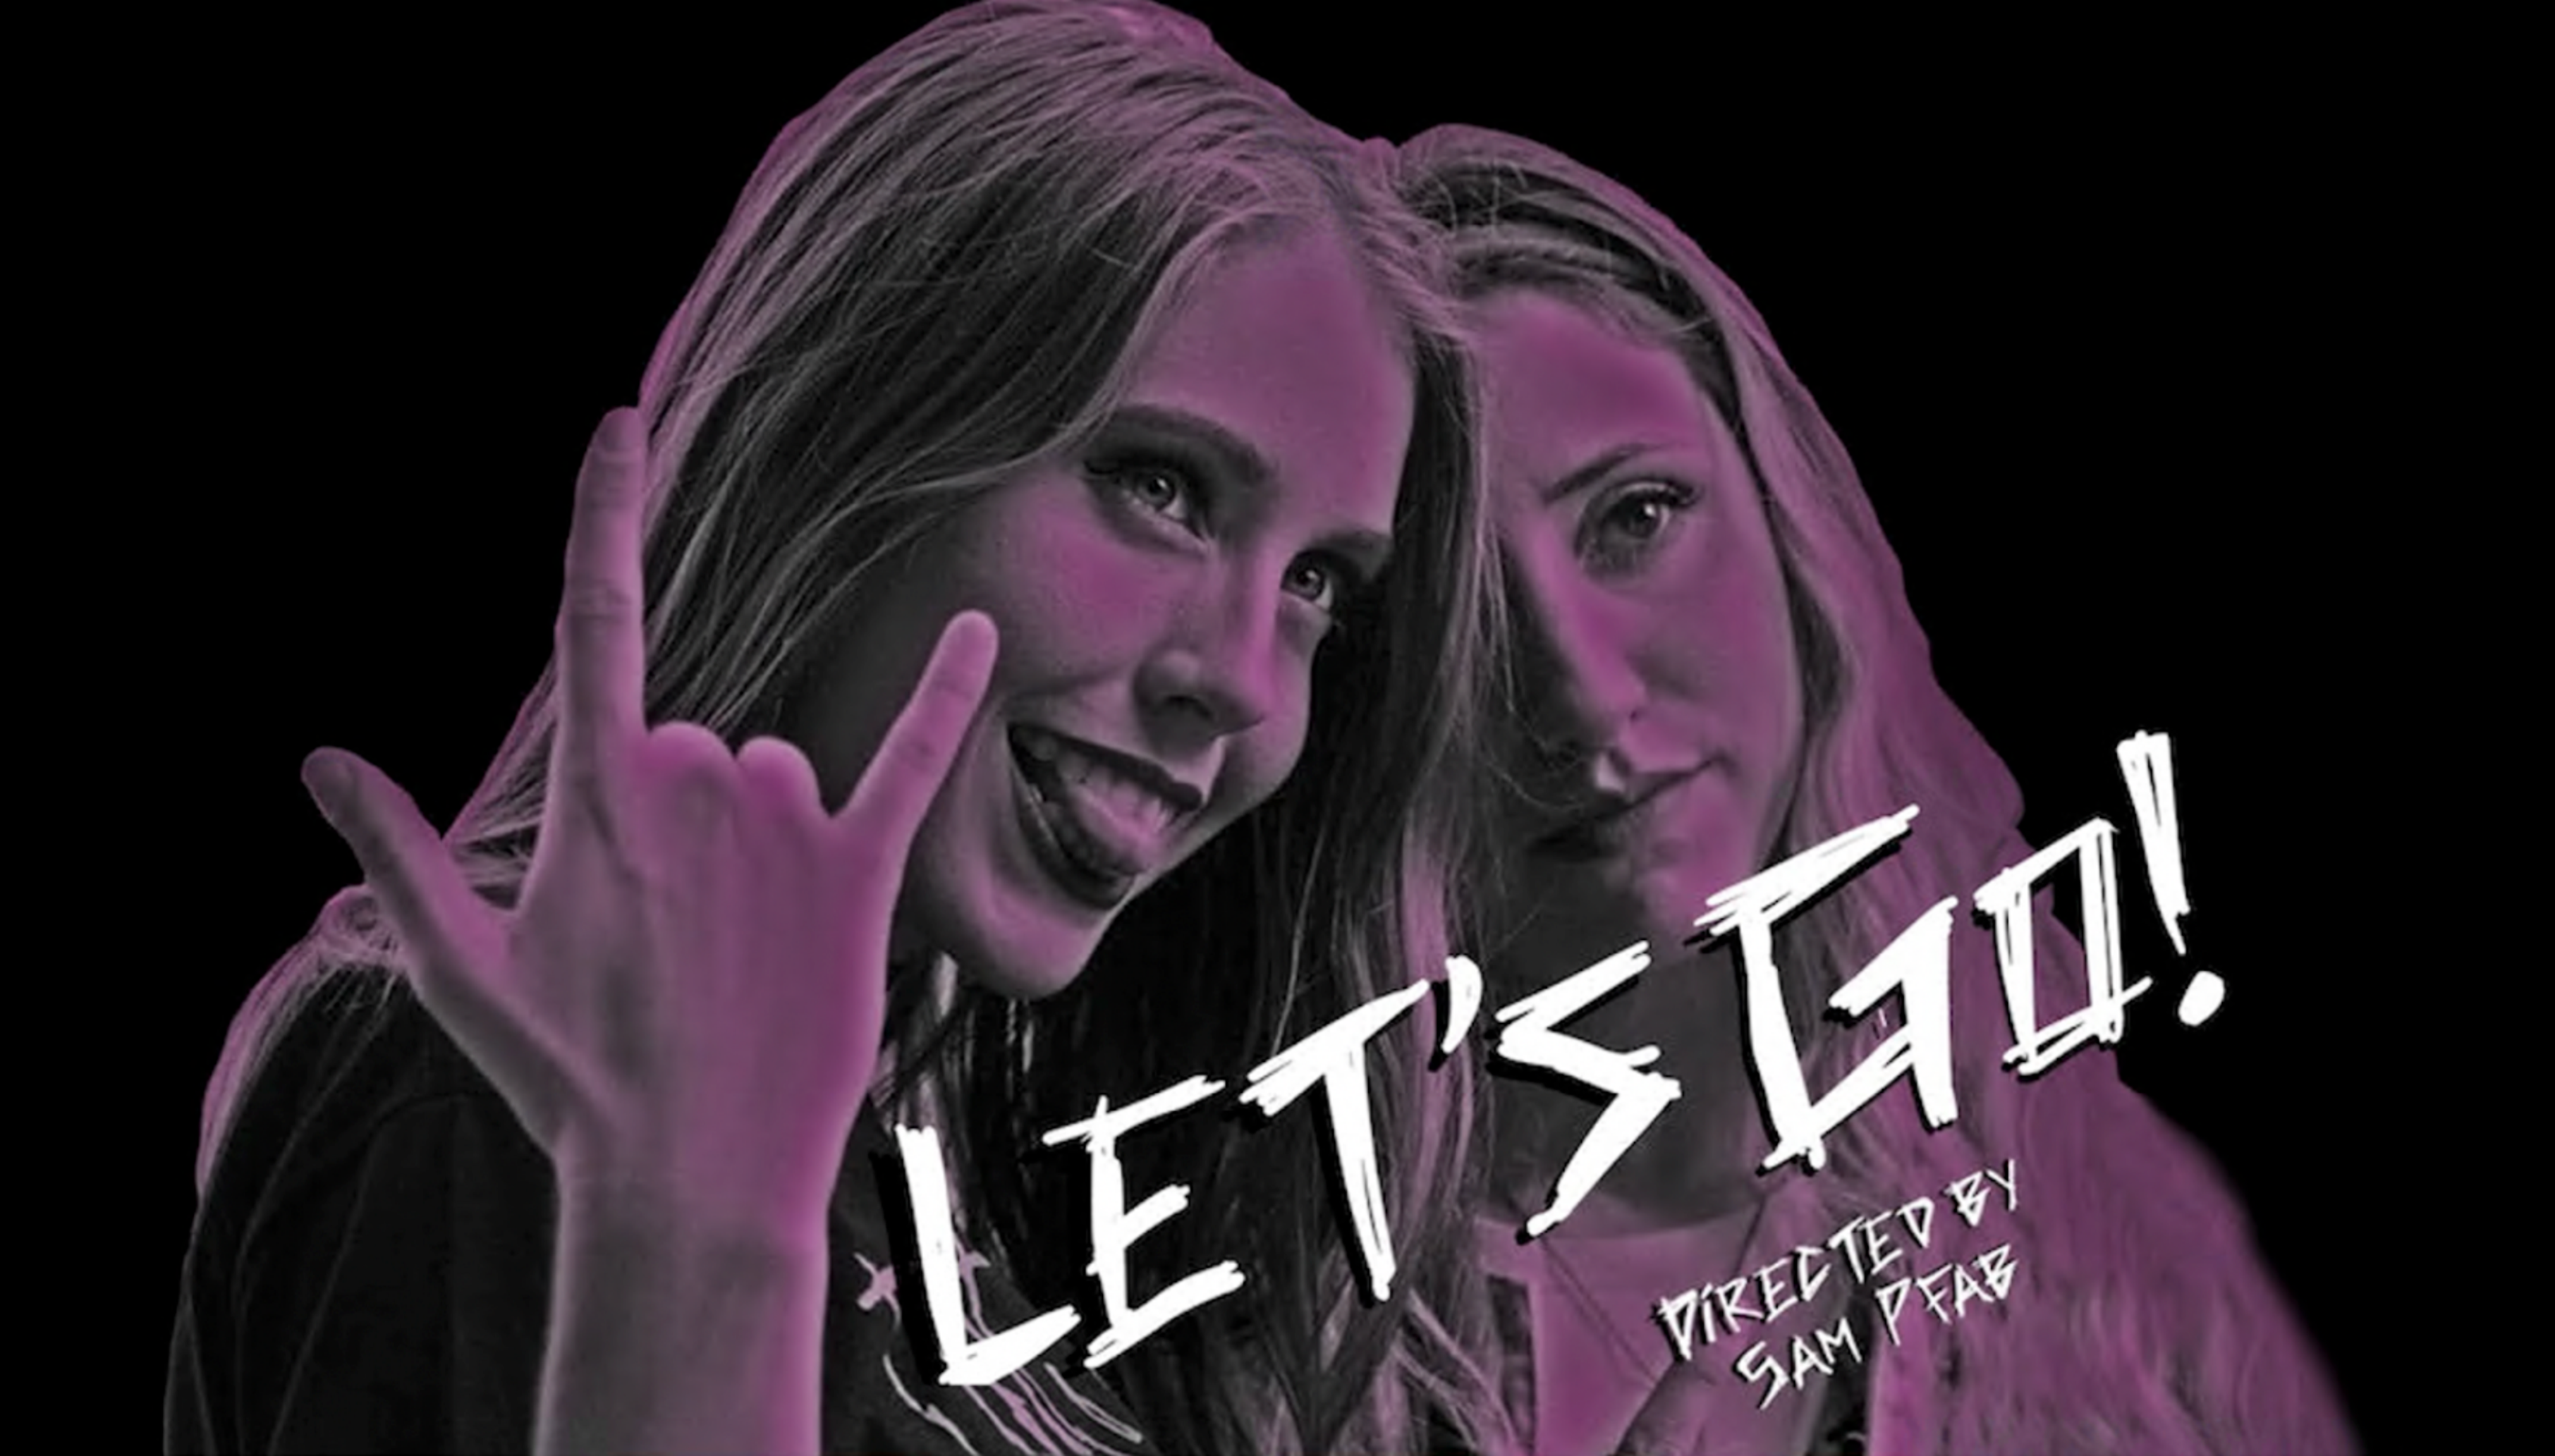
\includegraphics[width=8.5cm]{Figures/record_store_protest-2.pdf}
\vspace{-2em}
\caption{An example pair of image and human caption text from our crowdfunding dataset. The caption generated by the BLIP model and the actual human-generated caption of the image is below. 
\textbf{BLIP caption:} "Two women smiling with a hand gesture of rock and roll." 
\textbf{Actual human caption:} "Smash the glass ceiling. Destroy the patriarchy. Save the record store."}
\vspace{-2.5em}
\label{fig:image-womens-movement-patriachy}
\end{figure} 

Table \ref{tab:generated-caption-two-women} presents explanations generated by state-of-the-art multimodal models, including BLIP2 and LLaVA. While LLaVA \cite{liu2023visual} did generate contextually informed explanations of the input pair, it produced hallucinations, such as describing, “The image features two women standing next to each other, \emph{both holding their cell phones in their hands. They seem to be taking selfies},” when, in fact, there are no cell phones visible in the given image, nor are they taking selfies. To address this issue, we appended the input pairs in our dataset with the most relevant concepts from ConceptNet {\cite{speer2018conceptnet}}. This augmentation mitigated hallucinations as demonstrated in the generated outputs from example pairs in Table \ref{tab:generated-caption-two-women} in Appendix). This comparison highlights the value of multimodal analysis guided by external knowledge, which helps form more accurate cross-modal contextual connections. 

In this study, we examine the following two research questions: \\
\textbf{RQ1:} Can we enhance the cross-modal contextual congruence of the representations of multimodal content by incorporating external knowledge by learning to unveil subtle cross-modal semantic relationships? \\
\textbf{RQ2:} Do more contextually congruent representations help the models obtain more consistent and reliable predictive performance for the success of multimodal crowdfunding campaigns? 

Our work focuses on enhancing the cross-modal contextual congruence of representations of multimodal content for crowdfunding campaigns by incorporating an external Knowledge Graph (KG) (e.g., ConceptNet). As contextual congruence is defined as the association between multiple cues from various modalities (see Section \ref{sec:prelim}), we use ConceptNet, a commonsense knowledge graph with rich semantic knowledge of the world, to synthesize these diverse multimodal cues similarly that mirror human cognitive processes. We first take pairs of images and text from our dataset and generate embeddings using text and image encoders (i.e., via LLMs, LVMs). We generate captions for images to query the KG using BLIP \cite{li2022blip}. Then, our approach retrieves the most relevant concepts from ConceptNet based on semantic search. We learn knowledge graph embedding (KGE) models to generate representations of the resulting concepts. Initially, we learn multimodal data representations using bidirectional transformers. These representations are then fused with the KGEs through a fusion mechanism with linear and multi-head cross-attention layers to obtain enhanced knowledge-infused multimodal representations. 



Our findings indicate that knowledge-infused multimodal representations consistently outperform baseline models without knowledge. Further, we found that augmenting knowledge in the input of multimodal models bridges the semantic gap between the modalities, enhancing the congruence by bringing them closer. Error analysis (see \ref{sec:results-discuss} Section Results \& Discussion) reveals how external knowledge improves the capture of intended holistic multi-modal meaning. We demonstrate the contribution of knowledge to machine learning algorithms for computational analysis of crowdfunding campaigns, which provide an ecologically valid measure of success.

The contributions of this work lie in modeling a social and behavioral problem, such as successful crowdfunding campaigns, utilizing neural and symbolic models \cite{sap2022neural}. In so doing, we particularly tackle the problem of learning a contextually enhanced neural representation of multimodal content with external commonsense KG (i.e., symbolic) \cite{yu2022probabilistic}. This helps the model to better capture the holistic meaning across modalities, consequently improving the performance in predicting the success of multimodal marketing campaigns.

\begin{table*}[hbt!]
\vspace{-0.2em}
  \centerline{
    \begin{tabular}{p{0.8cm}p{1.3cm}p{14.6cm}}
    \toprule[2pt]
   \textbf{\centering Model} & \textbf{\centering Knowledge} & \textbf{Text Caption} \\
    \toprule[1pt]
    BLIP2 & \centering No & the cover of let's go with two girls posing in front of a purple background going for a protest. \\
    \toprule[1pt]
    BLIP2 & \centering Yes & The cover of a movie "let's go" talks about patriarchy in the record store. \\ 
    \toprule[1pt]
    LLaVA & \centering No & The image features two women standing next to each other, both holding their cell phones in their hands. They seem to be taking selfies or sharing a moment together. One of the women is making a funny face, adding a playful vibe to the picture. The other woman is simply enjoying the moment and being part of the fun. \\ 
    \toprule[1pt]
    LLaVA & \centering Yes & The image features two beautiful and majestic black women standing together, united in their quest to smash the glass ceiling and destroy the patriarchy. They are surrounded by record albums, highlighting their shared passion for music and the record store. Their powerful presence and determination to save the record store from any threat make for a compelling scene that showcases their strength and resilience in the face of oppressive societal norms. \\
    \bottomrule[2pt]
    \end{tabular}%
  }
% \vspace{-0.5em}
\caption{For the image and text pair (see Figure \ref{fig:image-womens-movement-patriachy}), the captions generated by the models BLIP2 and LLaVA when the model was prompted with the Image and Text with and without external Knowledge. The knowledge is extracted from ConceptNet as explained in section \ref{sec:explicit-knowledge} and appended to the prompt input to these models. 
%While t
\emph{The captions with generated knowledge show less hallucination.} See Table \ref{tab:generated-captions} in the Appendix for more examples.}
\label{tab:generated-caption-two-women}
\vspace{-2.5em}
\end{table*}

% \vspace{-1em} 
\section{Background \& Related Work}
\label{sec:related}
\vspace{-1mm}
We provide background information and review prior work in the following three areas: multimodal vision and language models, knowledge infusion in multimodal learning, and modeling marketing campaigns. 


\vspace{-3mm}
\subsection{Multimodal Models (Vision and Language)}
\label{sec:multimodal-transformers}
\vspace{-1mm}

% Pre-trained transformer-based unimodal models like BERT \cite{devlin2018bert}, ViT, Roberta, and 
The most recent multimodal VLMs, including LLava \cite{liu2023visual}, GPT4 \cite{openai2023gpt4}, BLIP2 \cite{li2023blip}, BLIP \cite{li2022blip}, CLIP \cite{radford2021learning} have demonstrated significant outcomes in capturing content, albeit with certain limitations, such as hallucinations \cite{li2023evaluating,cirik2022holm}. Early VLMs including ViLBERT \cite{lu2019vilbert}, LXMERT \cite{tan2019lxmert}, and MMBT \cite{kiela2019supervised} introduced two-stream architectures using pretrained unimodal models to generate representations fused in later layers. Initial semiotically-oriented research explored text-image relations between 
%text image relying on 
words and objects 
%(i.e., semiotics), 
by attempting to construct the holistic congruent meaning of the pair \cite{wu2014multimodal,manning1998understanding}. %For these image-text relations, s
Systems were proposed to identify and represent concepts in multimodal communications such as logico–semantic relations \cite{martinec2005system}. One taxonomy 
%was also developed to 
structurally represented these relationships utilizing cross-modal similarity \cite{marsh2003taxonomy}. As social media became prevalent, researchers created multimodal classifiers harnessing these text-image relations using a latent dirichlet allocation (LDA) model \cite{wang2014bilateral,chen2013understanding}.  
%Recently, researchers have paid  more attention to the prediction of the cross-modal correlation categories. 
More recently, researchers expanded the existing classification systems based on image specificity \cite{jas2015image}, emotion \cite{chen2015velda}, interrelation metrics \cite{henning2017estimating,otto2020characterization}, parallel and non-parallel \cite{zhang2018equal}, contextual and semiotic relations \cite{kruk2019integrating}, and the contribution of visual content \cite{vempala2019categorizing},  among other features. They used supervised learning to predict the \emph{cross-modal correlation} category using multimodal regression \cite{jas2015image} and multimodal classification \cite{chen2015velda,henning2017estimating,otto2020characterization,zhang2018equal,kruk2019integrating,vempala2019categorizing}. Despite the promising results of these predictive models, 
%there are still 
one persisting drawback 
%persists  in the existing studies concerning 
concerns the definition and classification of cross-modal correlation. As the existing definitions often include fine-grained relevant types of cross-modal correlation, it demands comparably fine-grained annotation effort 
%for annotation 
%of these fine-grained relationships 
to model the cross-modal correlation.
%which is challenging. 
Researchers built fine-grained datasets to attend to information from each modality and use them in multimodal classification \cite{chen2015velda,henning2017estimating,otto2020characterization,zhang2018equal,kruk2019integrating,vempala2019categorizing}.


\vspace{-2.9mm}
\subsection{Knowledge Infused Multimodal Learning}
\label{sec:knowledge-infusion-mm-learning}
\vspace{-1mm}
Large pretrained foundation models have become dominant paradigms in both vision and language (VL) modeling. Despite pretraining on large amounts of aligned VL data, usually from Conceptual Captions \cite{Sharma2018-qk}, COCO \cite{Ren2015-oq}, Visual Genome \cite{Krishna2017-xz}, and ImageNet \cite{deng2009imagenet} datasets, limitations persist in recent transformer-based approaches. They are restricted in the types of learned concepts and lack explicit information regarding commonsense knowledge, learning only surface-level characteristics.  For Language Understanding, researchers have recently employed knowledge-enhanced approaches using knowledge graphs for several tasks, including Language Modeling \cite{yasunaga2022deep,zhang2022greaselm,Logan2019-tk,Lu2021-xe,kursuncu2020kil}, Natural Language Inference (NLI) \cite{Ni2021-db}, Language Generation \cite{Yu2022-uv,peters2019knowledge}, E-BERT \cite{Wu2022-ah}, ERICA \cite{Qin2020-et} ERNIE \cite{Zhang2021-ov}, ERNIE-NLI \cite{Bauer2021-rv}, LUKE \cite{Yamada2020-zc}.  

% \textcolor{red} {This paragraph is a total disaster---so bad I can't even begin to edit. 
% Vision Understanding researchers have investigated tasks such as 
Visual Commonsense Reasoning (VCR) 
%was an area of interest to researchers to 
appealed to researchers attempting to incorporate external knowledge in VLMs.  
%where t
They created a unified representation of scenes by merging scene graphs and structured information from ConceptNet to enhance visual understanding and explainable reasoning \cite{Zareian2020-vw,Pan2022-jd}. 
%but mostly these works are based on  to show how 
% Even these large pretrained models are semantically inconsistent and need to be trained with large KG models. 
While the majority of the multimodal knowledge-enhanced 
approaches were employed in prior work (e.g., for Visual Question Answering (VQA)) \cite{Garderes2020-gx,Marino2021-sn,Wu2022-lj}, they were limited to keyword-based entity matching to extract explicit knowledge. In another vein, representations of scenes for autonomous driving have been enhanced using knowledge-infused learning \cite{wickramarachchi2022knowledge,wickramarachchi2021knowledge}.
%It can be also seen to reduce the hallucination models, 
Further, as hallucination has been a significant limitation of LLMs, LVMs, and VLMs, researchers utilized knowledge-enhanced models to address this issue, again for VQA \cite{Chen2023-mf}. Our work differs from previous approaches in that we jointly reason over both implicit and explicit knowledge extracted through semantic search and infused into the model. 
% TP:% unlike \cite{Gui2021-ax} implicitly as sometimes it is not enough for the model due to limited context length at the input. 
% Hence after we extract semantically similar concepts 
% %and  motivated by \cite{Kursuncu2019-ha} 
% infusing knowledge in the model help the model learn contextually congruent and coherent representations of social media content inclusive of both modalities. 
% This is in contrast to previous approaches that have focused on either implicit or explicit knowledge, or on single modalities. 
% Our approach is more comprehensive and allows us to learn more accurate representations of social media content, measured 
% %as can be seen with the 
% by a reduction of Modality Gap.  This implies that the representations are consistent with the intended interpretation.
% %context in which the content was created. 
% %This is important because it allows us to better understand the meaning of the content and to use it in a variety of applications.

\vspace{-1em}
\subsection{Modeling Crowdfunding Campaigns}
\label{sec:modeling-social-media}
\vspace{-1mm}
Marketing materials are often generated to promote an entity (i.e., organization, product, person) and 
%persuade the audience about the information being conveyed. 
instigate audience action. Online platforms including social media and crowdfunding have been a focus area for marketing campaigns due to its reach to the masses in real time \cite{kursuncu2019predictive}. Crowdfunding platforms, such as Indiegogo and Kickstarter %are an effective way to reach the masses and seek
seek venture capital from the general public.
%contributions to fund their venture. 
% \textcolor{red} {Disaster: 
% similar to other cam-paigns (e.g., political campaigns), constitute a genre of strategic communication with readily measurable outcomes. The majority  of emerging brands originate as startups in crowdfunding platforms including Kickstarter and Indiegogo, as it is an effective way of reaching masses and seek contributions to finance their venture \cite{Carradini2023-ka}. 
Between 2009 and 2023, over seven billion dollars have been pledged for the campaigns on Kickstarter. Some of the emerging brands such as Oculus \cite{Carradini2023-ka} originated from these platforms.
% The success of any marketing campaigns depends on its ability to evolve with the changing needs of consumers, and to provide an engaging and informative experience. However, the complexity of such marketing campaigns poses a computation challenge for machine understanding. The benefit of a strategic approach for a crowdfunding project is demonstrated by the fact that many campaigns fail to obtain their funding goals.  For example, Kickstarter has currently a \%38.76 acceptance rate, which is the ratio of campaigns getting fully funded. Carradini et. al.\cite{Carradini2023-ka} %analyzed successful and unsuccessful campaigns and 
These campaigns have a relatively low success rate. For instance, Carradini et al. \cite{Carradini2023-ka} 
%analyzed successful and unsuccessful campaigns and  
found that \%38.76 of the Kickstarter campaigns were fully funded relative to unsuccessful campaigns.   Successful campaigns featured more images and links. Yet, the majority of crowdfunding studies focused primarily on textual content, 
%To the best of our knowledge, research on computational analysis of multimodal crowdfunding campaigns has been inadequate. 
and often followed a more standard data science approach. 
%using unimodal resources.
%, specifically for success prediction of campaigns. 
Researchers \cite{Mitra2014-ly} analyzed the textual data in Kickstarter campaigns, extracting linguistic features with phrases (i.e., n-grams) and other control variables using a logistic regression model. 
%There have been very few research utilizing 
Another study built models to characterize the persuasive strategies in crowdfunding (Kiva) campaigns using semi-supervised textual RNNs \cite{yang2019let}. This research topic of multimodal learning
%approach for 
specifically for modeling crowdfunding campaigns and their success has not received adequate attention from the researchers \cite{Palmieri2022-ch,Carradini2023-ka}. Researchers \cite{cheng2019success} developed one of the few predictive models for multimodal crowdfunding campaign success (MDL-TIM) (we use this model as a baseline ---see Section Methods---). 
Because marketing campaigns are often multimodal, congruence in the promotional multimodal content is likely critical for effectiveness. The crowdfunding application provides an ideal domain for addressing the contextual congruence between modalities, providing both ample data and a measure of successful interpretation.
%The general challenges in analyzing multimodal content also persist for crowdfunding campaigns including facilitating contextual congruence between modalities to capture the true meaning. 

In contrast to the above approaches, we use commonsense knowledge to reduce the gap between modalities to 
%helps in better 
improve cross-modal congruence. Our work differentiates itself by utilizing both implicit (data-driven) and explicit (knowledge-driven) information fused in multimodal learning, which provides more contextually congruent representations and better performance in our downstream task.



% \vspace{-2em}
\section{Preliminaries}
\label{sec:prelim}
\vspace{-1mm}
Multimodal marketing materials are often strategically designed to promote various entities, products, brands, or individuals, aiming to persuade an audience of their qualities and ultimately influence them to take action. For crowdfunding, this desired action is for users to commit as "backers," contributing financially to support the campaign before its deadline. The decision-making process for potential backers involves synthesizing and evaluating both textual and visual content, requiring an understanding of how these modalities interact. This multi-sensory input from different modalities requires forming cross-modal semantic connections to capture the holistic meaning. These semantic connections spanning both modalities facilitate a contextually congruent information environment that enhances cognitive processing, enabling humans to process information more efficiently and effectively \cite{laurienti2004semantic,spence2011crossmodal}, thus increasing the persuasiveness of the campaign message \cite{schubert2021multimodal}. 
 
\vspace{-1em}
\subsection{Cross-Modal Contextual Congruence}
\label{sec:context-congruence}
\vspace{-1mm}

Contextual congruence refers to the associations between multiple sensory cues from different modalities known to enhance human response accuracy \cite{laurienti2004semantic,spence2011crossmodal}. Recent research suggests that contextual congruence in cross-modal space facilitates the selection and processing of semantically related information from different modalities \cite{almadori2021crossmodal,laurienti2004semantic,letts2022evaluating}. Capturing holistic meaning is essential for predicting human response to multimodal crowdfunding campaigns. However, multimodality challenges computational modeling, as the semantic cues span across modalities to construct meaning. 
While the human brain adeptly forms these meaningful semantics connections between modalities, mimicking this capability for machines has been a complex issue. 
Our approach aims to achieve this capability to discern contextual congruence by utilizing external knowledge from ConceptNet to enhance the multimodal data representations in learning. 

\vspace{-2mm}
\subsection{Dataset}
\label{sec:dataset}
\vspace{-1mm}

We have chosen the Kickstarter crowdfunding platform for its promotional multimodal content, where we have a valid outcome measure with a relatively large N. We utilize a dataset from Web Robots \cite{robots2018kickstarter} that collects data on  Kickstarter campaigns including attributes such as categories, goals, amount funded, the backers count, country, project type, and project URLs, among others. The dataset will be made available and fully comply with the FAIR principles \cite{force11}.

Kickstarter is an online crowdfunding platform where creators, entrepreneurs, designers, and artists, initiate promotional campaigns to seek resources for their creative projects in various categories. A campaigner introduces the concept behind their project in a project description. To back up their campaign, they frequently post videos, images, and text ads. Each project has a funding target with a deadline for a successful campaign. A project only receives the funds if it achieves or surpasses its funding target by the deadline going by the \textit{all-or-nothing} principle. 

We chose a one-year time frame between June 2021 and May 2022, and randomly sampled 75,810 Kickstarter projects. A project is considered successful if it reaches its funding target by the deadline. Our binary outcome variable represents whether the project was successful or unsuccessful. In our dataset, 60.63\% were unsuccessful while 39.37\% were successful. 



% \vspace{-1.5em} 
\section{Exploratory Analysis}
\label{sec:exploratory}
\vspace{-1mm}

We examine the importance of contextual congruence by exploring the semantic distance between text and image modalities and whether utilizing external knowledge from ConceptNet will bring this distance closer and better reflect their semantics, as explained below. More specifically, we measure contextual congruence in multimodal content using the semantic distance between the separate image and caption (text) representations, as this distance is expected to be shorter in a relatively congruent multimodal representation \cite{mandera2017explaining,frank2017word,beck2011congruence,maki2004semantic}. We can then demonstrate how external knowledge can enhance and contextualize the representations to bridge the semantic gap between the modalities. In doing so, we can better predict the success of crowdfunding campaigns. 


We generated the captions for image modality using BLIP to demonstrate this idea, resulting in a textual description for each modality as text. We used semantic search (see Section Knowledge Retrieval) to extract the most relevant concepts for both text and image captions. Then, we appended these concepts to the input, which is a pair of text and image captions, to generate representations using BERT. We performed clustering analysis using DB-SCAN over the text and image captions --- we validated that the clusters represented text and image modalities.--- Our goal here is to show how the centroids of each cluster change when external knowledge is included in the input. Hence, we ran two clustering algorithms, with and without external knowledge.

\begin{figure}[hbt!]
\vspace{-1.1em}
  \centering
  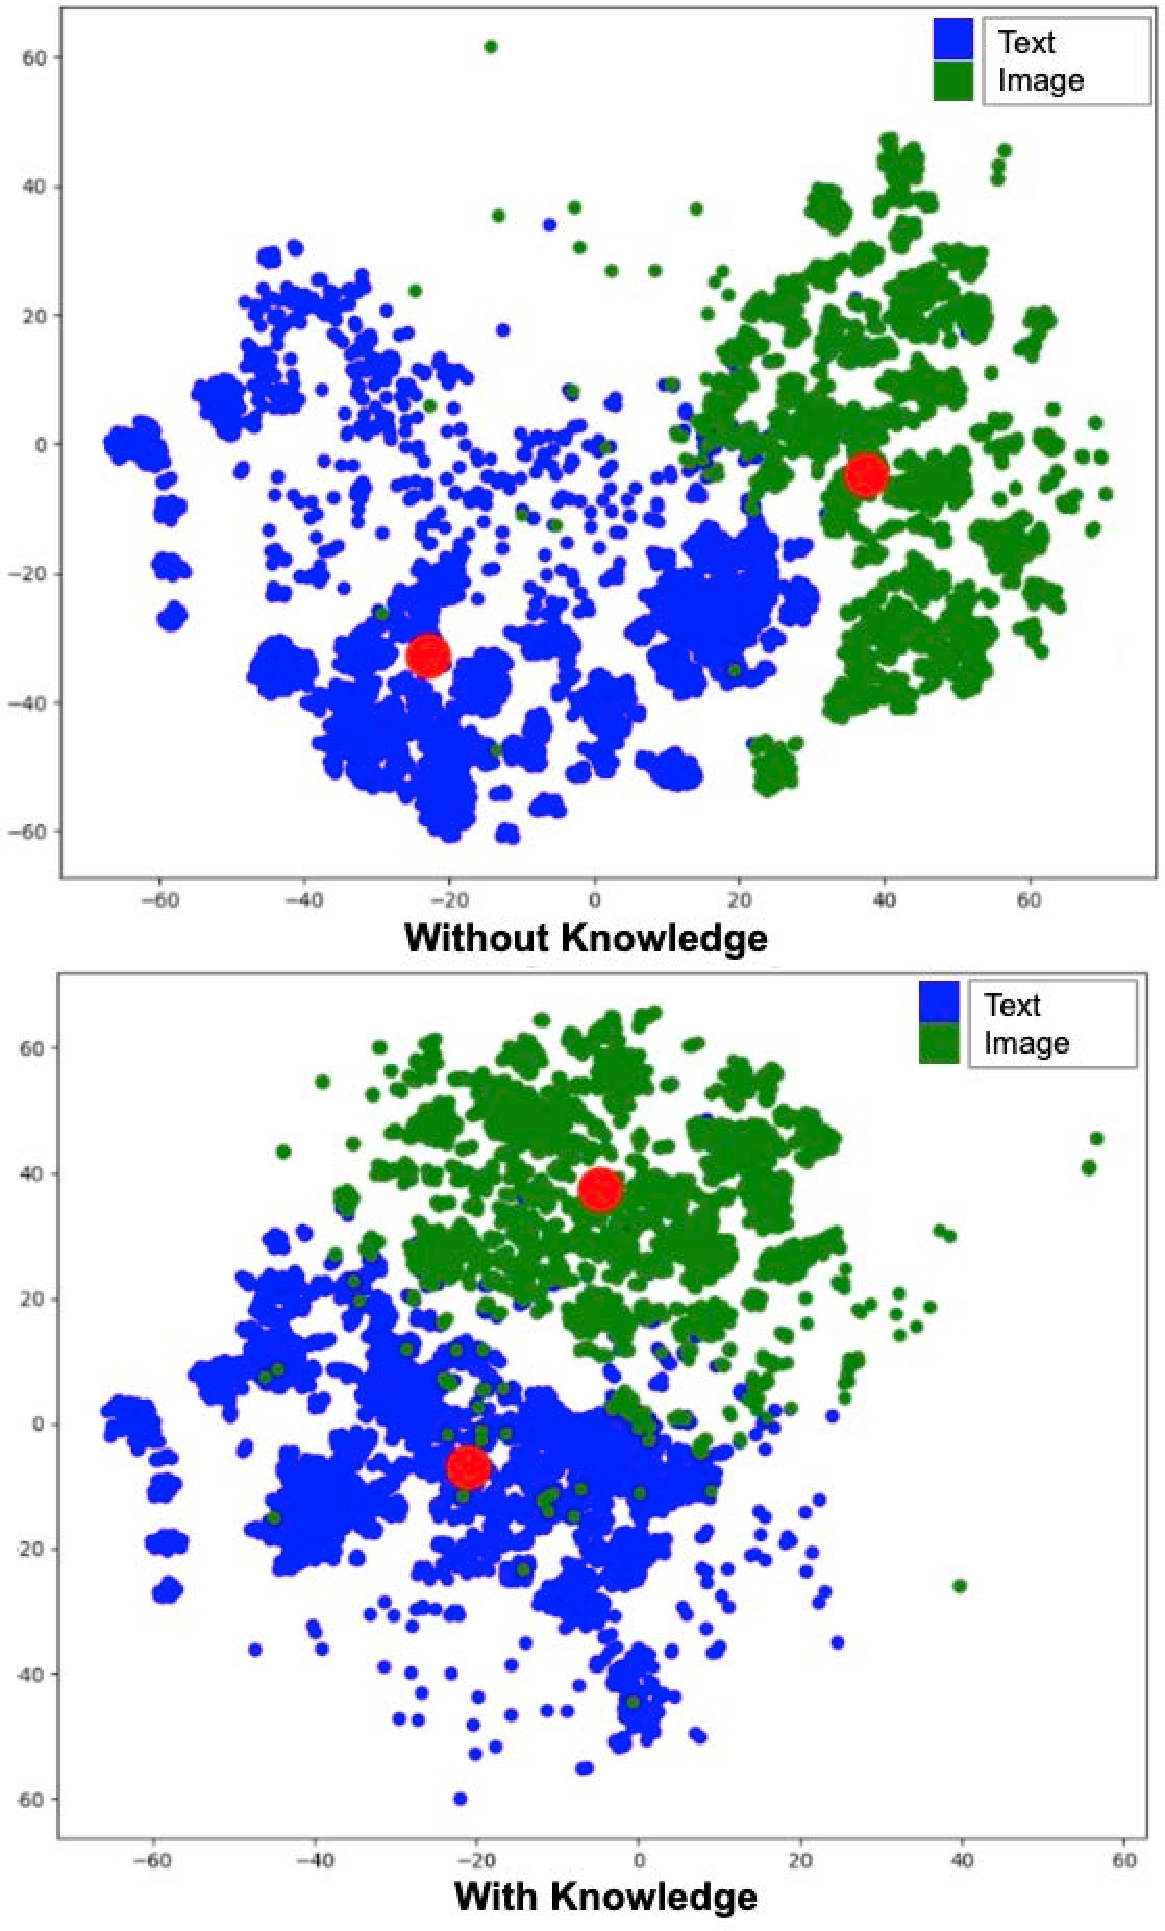
\includegraphics[width=8cm]{Figures/congruence_cluster_vertical.pdf}
\vspace{-1.5em}
\caption{t-SNE visualization of text and image caption (BLIP) embeddings as two clusters. The red dots represent the centroids in each cluster. The two clusters get denser and the distance between the text and image clusters reduces when we include concepts that we extracted from ConceptNet based on text and image captions.}
\vspace{-1.2em}
\label{fig:embds-cluster}
\end{figure} 


Figure \ref{fig:embds-cluster} shows t-SNE visualizations of the text and image clusters created with and without external knowledge. The upper clusters (without knowledge) are more scattered, whereas the lower clusters are denser. The centroids in the clusters with knowledge are also closer to each other, demonstrating the semantic distance is reduced because it can better reflect their semantic relationships. We ran the same experiment with different sizes of data points; 
%and our observation did not change as 
the clusters consistently got denser and centroids closer (see Figure \ref{fig:context_congruence_across_data_size} in the Appendix).
We also measured semantic similarity using cosine for each text-image pair in these clusters and created their density plots (see Figure \ref{fig:density-plot}). 
%In other words, rather than measuring the semantic distance between centroids, we measured the similarity between image and text modalities in a pair. From figure 
Figure \ref{fig:density-plot} shows
%we can also observe that 
that the similarity between text and image modalities increased by about 9.9\%.


\begin{figure}%[hbt!]
  \centering
  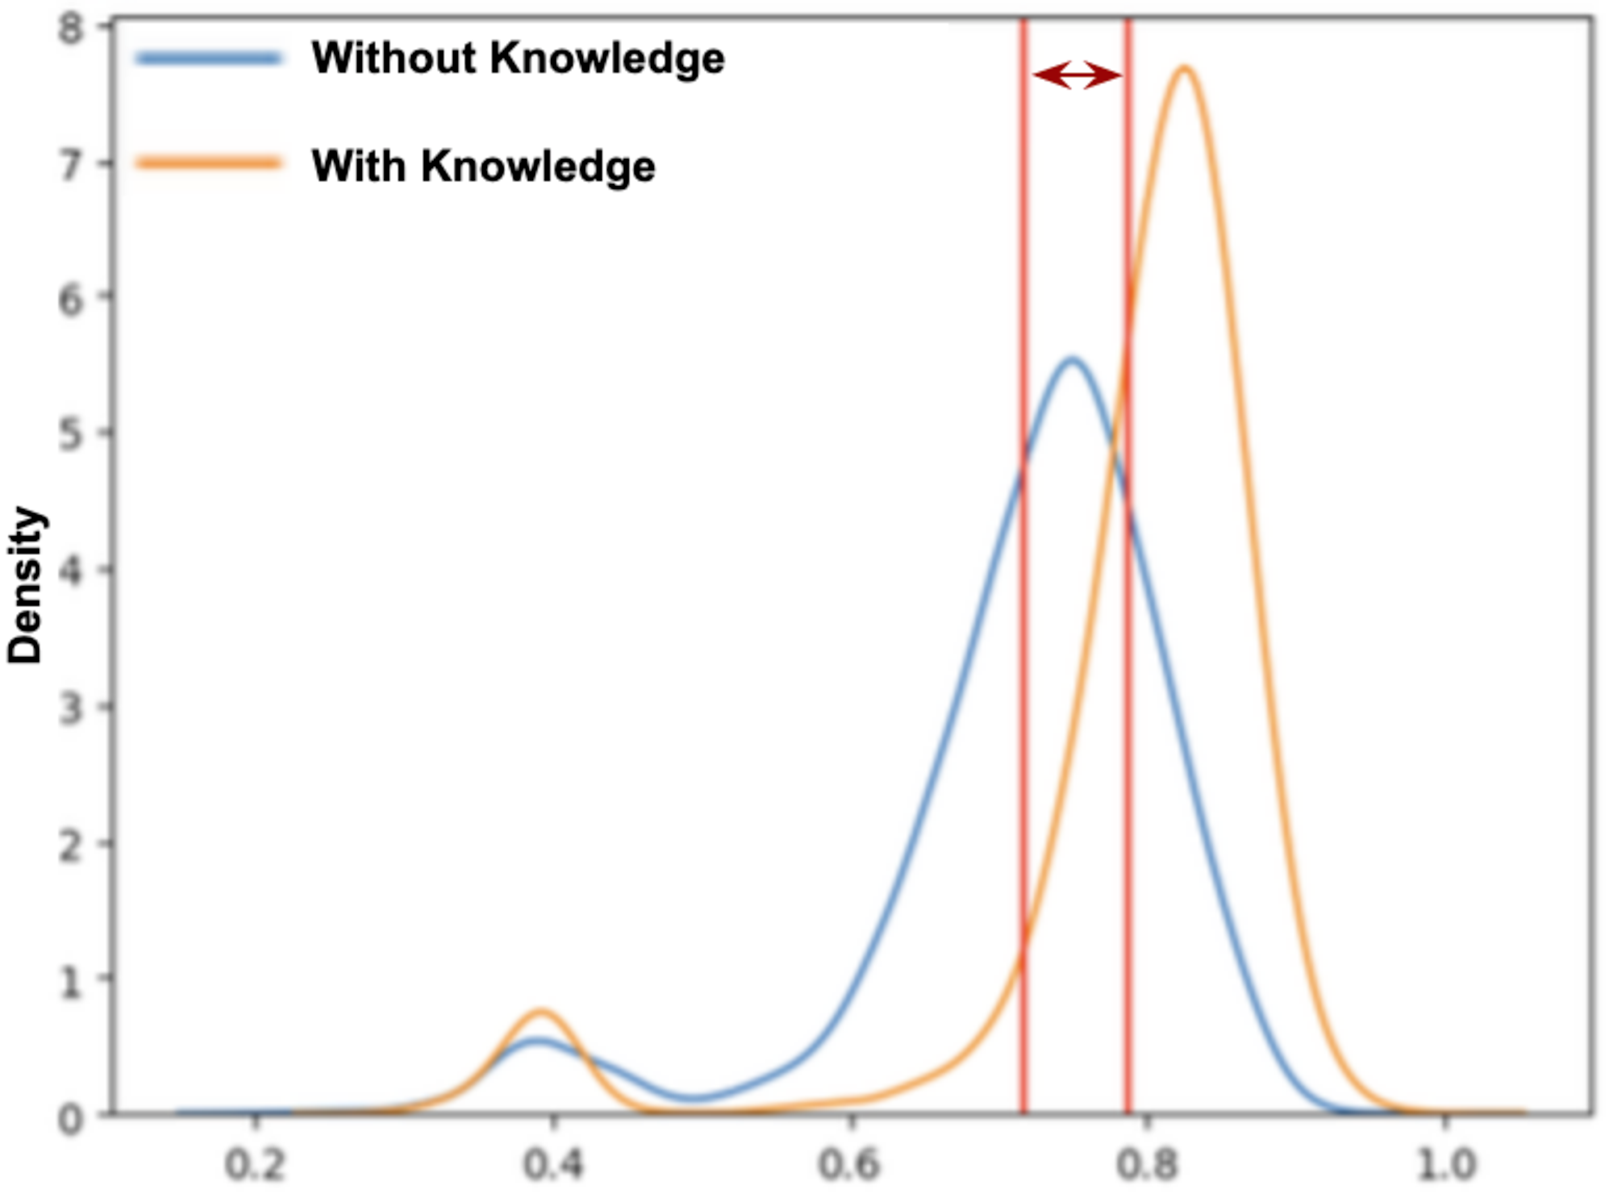
\includegraphics[width=7.8cm]{Figures/density-plot.pdf}
\vspace{-1em}
\caption{Density Plot demonstrates the difference between the similarities (cosine) of the image and text embeddings with and without knowledge. The inclusion of knowledge in the input gets text and image modalities closer by about 9.9\%.}
\vspace{-2.3em}
\label{fig:density-plot}
\end{figure} 


In addition, as we pair image and text modalities (see Figure \ref{fig:image-womens-movement-patriachy}),
% with the 
%human-generated 
% caption, 
the VLMs recognize relationships between modalities. %capturing the meaning to an extent while 
However, hallucinations are amplified by making non-existent connections and nonfactual information. Explicit knowledge from KGs can facilitate 
%the contextualizing and 
factual grounding.
%to capture the true meaning. 
We queried the KG to extract relevant concepts and simply include these with the pair of images and text as input for the VLMs such as Llava and BLIP. 
%We observe that the hallucinations are mitigated. 
This mitigates hallucinations. 
%For instance, in our example in 
As shown in Table \ref{tab:generated-caption-two-women}, the generated caption with knowledge does not include hallucination while containing contextual relationships from both the image and human caption.
%and is more contextually meaningful as the image and human caption are embedded in the meaning. The reader may find more 
Other examples appear in the appendix with generated captions (see Table \ref{tab:generated-captions}). 
These observations demonstrate the potential contribution of external knowledge to create more congruent multimodal representations by forming contextual relationships between modalities.  


\begin{figure*}[hbt!]
 % \vspace{-4em}
    \centering
  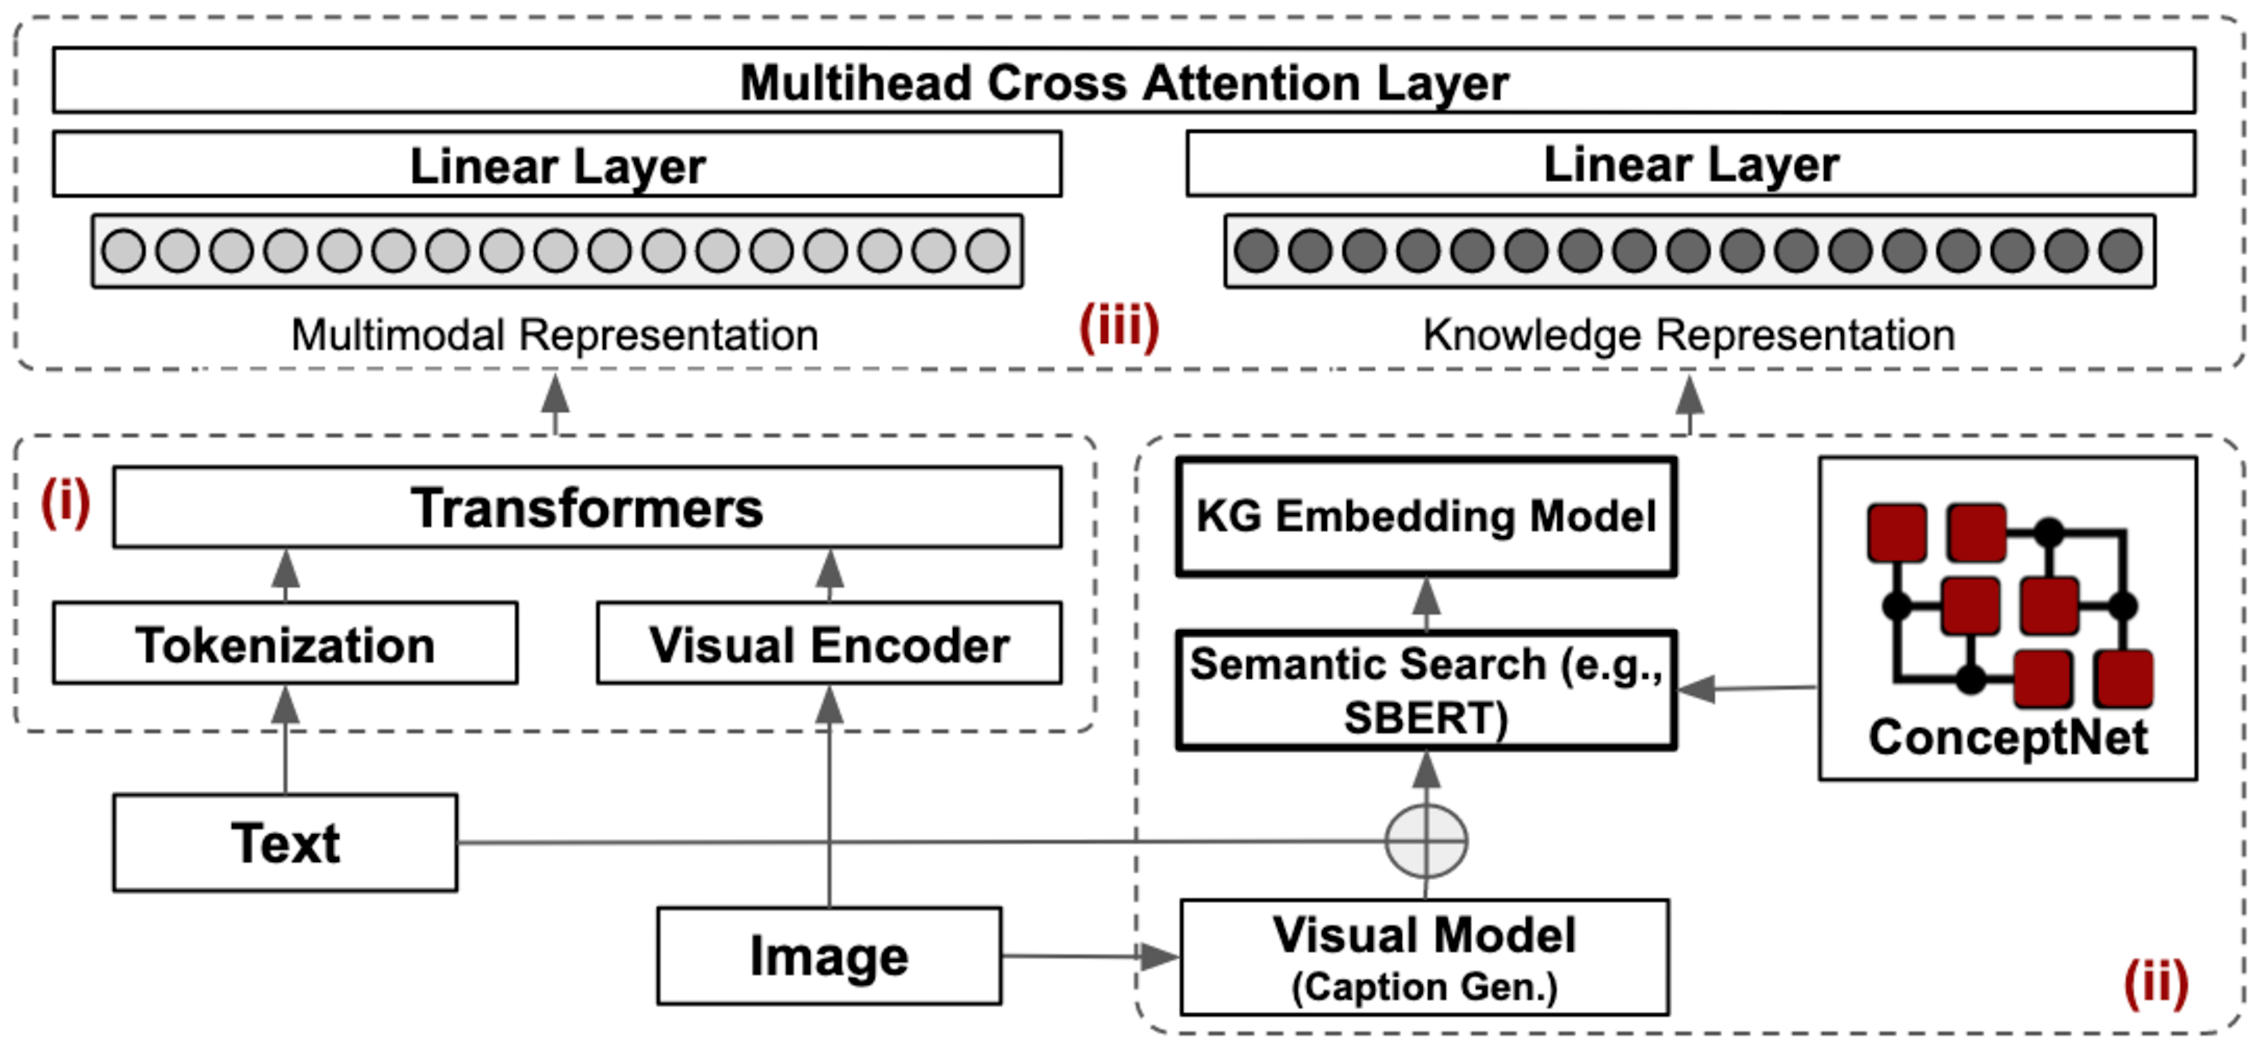
\includegraphics[width=17cm]{Figures/diagram.pdf}
\vspace{-0.8em}
\caption{Our approach consists of three main components: (i) multimodal learning, (ii) knowledge retrieval and representation, and (iii) Knowledge Fusion Layer. The Retrieval component identifies the most relevant concepts from ConceptNet. The concepts' KG embeddings are generated. The knowledge fusion layer fuses the multimodal representations with knowledge embeddings followed by Softmax.}
\vspace{-1em}
\label{fig:architecture}  
\end{figure*}


% \vspace{-0.8em} 
\section{Methods}
\label{sec:methodology}
\vspace{-1mm}

As shown in Figure \ref{fig:architecture}, our models incorporate external knowledge from ConceptNet in a multimodal learning framework to predict the success of a crowdfunding campaign. We formulate this as a binary classification task, where the goal is to determine whether a campaign will be successful. We use a supervised multimodal learning framework \cite{kiela2020supervised} to learn multimodal representations. We devise a knowledge retrieval component that extracts the most relevant concepts from ConceptNet. We trained Knowledge Graph Embedding (KGE) models for knowledge representations as described in the Section for Knowledge Retrieval and Representation. Knowledge representations of the selected concepts are then generated using the KGE models. Then, we fuse the multimodal representation with the knowledge representation to obtain a knowledge-infused representation. This enhanced representation is then input to the classification layer to predict the campaign outcomes. 

In this study, we opted to use experiments with smaller language models such as BERT and RobertA, and visual models such as ResNet and ViT, which have demonstrated performance comparable to or exceeding larger models. While our exploratory analysis included more substantial models, including BLIP2 and LLaVA, we leave extensive experiments with such larger models as future work due to the required prohibitive computational costs. This strategic choice also allows us to focus on the performance of smaller but lean models as competitive baselines before scaling up to much larger and more computationally demanding models.

\noindent\textbf{Baselines.} We compared our approach with four different baselines. We used a baseline approach from recent literature for predicting crowdfunding success, MDL-TIM \cite{cheng2019success}. In addition, we used \cite{kiela2020supervised} as-is as another baseline model. Then, we created two more baselines that are variants of \cite{kiela2020supervised} by changing the text and image encoders. 
All models were trained/fine-tuned on the dataset with the same experimental settings (see Section {\ref{implementation-details}).

\vspace{-2mm}
\subsection{Problem Formulation}
\vspace{-1mm}
Our dataset contains data points  ($d_i$) consisting of pairs of image ($v_i$) and text ($t_i$) with binary labels ($a_i$); $d_i = {(v_i,t_i,a_i)}$ for $i=1...n$.
% ($a_i$); $d_i = {{(v_i,t_i,a_i)}^s}_{i=1}$
%, where $v_i$ represent the $i^{th}$ marketing image, $t_i$ represent the $i^{th}$ marketing caption of the image and $a_i$ represents its target, if the campaign was successful or not, if funded it's represented by $a_i = 1$ else $a_i = 0$
Our target classification feature is %determined 
based on whether a campaign is successful; in other words, whether it has reached its funding goal within a given timeline.
%binary response variable representing whether the project is funded or not funded. If a campaign achieves its target within the timeline, its successful and funded. 
Hence, our problem is to determine how likely a given marketing campaign with multimodal content (e.g., text, image) on a crowdfunding platform will be successful.
%by capturing contextual connections through the incorporation of knowledge representation in multimodal learning. 
We denote the knowledge graph as $K_g$ and the set of concepts as $C = {\{c_1, c_2, c_3, ....., c_n\}}$.
% Provide some examples for these concepts.


\vspace{-2mm}
\subsection{Multimodal Learning}
\label{mmbt-kil-model}
\vspace{-1mm}
Given each pair of image and text ($v_i,t_i$), we follow \cite{kiela2020supervised}, 
%to learn a multimodal representation 
because of the modular and flexible framework as the text and image encoders can be replaced and fine-tuned. Specifically, we jointly fine-tune the pretrained text (e.g., BERT, RoBERTa) and image encoders (e.g., ViT, ResNet) 
%that we experiment with over our dataset, 
using a bidirectional transformer. We initialize the bidirectional transformers with the fine-tuned text encoders and learn weights $W_n \in \mathbf{R}^{P\times D}$ to map each image ($v_i$) embedding to the token input embedding space. 
% These multimodal embeddings and the knowledge embeddings are concatenated and then a joint representation is learned in the multi-head cross attention fusion layer. The model is trained with a cross-entropy loss.

\vspace{-1.5mm}
\paragraph{Vision Encoder.}
\label{vision-encoder}
%The last fully connected layer of a pre-trained convolutional neural network is often used in computer vision \cite{azizpour2014cnn}, where the output comes from a pooling operation over feature maps. 
% We examine the impact of having the pooling generate N different picture embeddings as opposed to a single output vector, which is different from a traditional convolutional neural network. In this instance, w
We experiment with two types of vision encoders: ResNet-152 \cite{he2015deep} and Vision Transformers \cite{dosovitskiy2021image} model with average pooling over \begin{math} K \times M \end{math} grids in the picture, producing \begin{math} N = KM \end{math} output vectors with a total of 2048 dimensions for each image. As suggested in \cite{kiela2020supervised}, we resized, center-cropped, and normalized the images.


\vspace{-1.5mm}
\paragraph{Text Encoder.}
\label{text-encoder}

Our approach utilizes base-uncased BERT \cite{devlin2018bert} and RoBERTa \cite{liu2019roberta} as our multimodal framework (MMBT) is based on bitransformers. Contextual embeddings are created by adding distinct D-dimensional segments, location, and token embeddings. We learn weights $W_n \in \mathbf{R}^{P\times D}$ to project each of the $N$ image embeddings to $D$ dimensional token input embedding space: 

\begin{equation}
    I_n = W_nf(img,n)
\end{equation}

where $f(·, n)$ is the \textit{n}-th output of the image encoder’s final pooling operation. We use 0-indexed positional coding, i.e., we start counting from 0 for each segment. 

\subsection{Knowledge Embedding Models}
\label{sec:knowledge-embedding-models}

Knowledge graph embeddings, also known as knowledge graph representation learning, are techniques used to represent entities and relationships as dense, low-dimensional vectors. These embeddings capture the semantic relationships and similarities between entities and allow for efficient computation and reasoning in knowledge graph-based tasks. In our study we refer to the knowledge graph as $K_g$. Each triple in $K_g$ is represented as $(h,r,t)$ where the entities relation, head and tail are represented as  $h$, $r$ and $t$ respectively.

\textbf{TransE} \cite{bordes2013translating} is a translational energy-based model that represents entities and relations as vectors of the same Euclidean space $R^d$. For a given triple, score function is defined as $f_r(h,t) = -||h+r-t||_{l_1,l_2}$.
% In terms of vector computation it could be represented as or $ h + r \approx t$. 
% TransE performs linear transformation using the following scoring function:

% \begin{equation}
% f = -\lVert h+r-t \rVert_{\frac{1}{2}}
% \end{equation}
\textbf{RotateE} \cite{sun2019rotate} is a translational based model that represents entities and relations in complex vector space $C^d$ and defines each relation as an element-wise rotation from the head entity to the tail entity. The score function is formulated as $f_r(h,t) = - ||h\odot r - t||$, where $\odot$ is the Hadamard (or element-wise) product. 

\textbf{DistMult} \cite{yang2014embedding} DistMult is a semantic-matching model, where the score of a triple can be computed as the bilinear product which is represented as $f_r(h,t) = h\times r \times t$ where $e_h,e_t \in R^d$ and $r \in R^{d \times d}$. Here, restricting $R$ to a diagonal matrix, the score is computed as $f_r(h,t) = h\times diag(r) \times t$.
% In DistMult, every relation $r$ is represented by a diagonal matrix $M_{r}  \in {R}^{{d} \times {d}}$ and a triple is scored as $f(h,r,t) = {e_h}^TM_rE_t$ where $e_h,e_t \in R^d$.
% and a triple is scored as:

% \begin{equation}
% f(h,r,t)= e^{T}_{h} M_{r} e_{t}
% \end{equation}


\vspace{-0.8em}
\subsection{Knowledge Retrieval and Representation}
\label{sec:explicit-knowledge}
\vspace{-1mm}
% Multimodal marketing content often has rich complementary information across modalities 
%that are complementary to each other and 
% The implicit knowledge in pretrained models fails to capture these nuances. 
%Common Sense KGs express real-world truth.  
We generated a text caption for images using multimodal LVMs for knowledge retrieval. BLIP \cite{li2022blip} performs better than other models and is sufficiently accurate in representing the image content. The text and the generated caption of the image are combined and input into the semantic search module. For semantic search, we utilize Sentence-BERT \cite{reimers2019sentence} to search efficiently and find the most semantically meaningful matches (e.g., $top-k$) between  KG concepts and content input. Sentence-BERT was trained with a regression objective function (e.g., mean squared error) and a siamese network architecture over a sizable natural language inference (NLI) data, which enables efficient inference and semantic search capabilities. 
%As per 
Due to its comprehensive coverage of commonsense knowledge, we use ConceptNet \cite{speer2018conceptnet} as our KG. In order to retrieve the most relevant concepts, Sentence-BERT computes the similarity scores, resulting in the $top-k$ concepts ($c_i$) that are semantically similar to the input text and image caption pairs ($v_i,t_i$). In our experiments, we empirically selected $k= 10$. 
%To define the similarity score between the pair of ${v_i,t_i}$  and the concept $C_i$, we use cosine similarity as a metric to rank the most related entities.

% \begin{equation}
% Cosine(x,y) = \frac{x \cdot y}{|x||y|}    
% \end{equation}

% These concept sets $C_{Vi}$ and $C_{ti}$ represent respective modalities, in this case, image and text, respectively, from the KG. We retrieve the $top-k$ concepts relevant to the image and text. These top entities retrieved are represented by ${C_i}^k$. 
As we obtain the most relevant concepts from ConceptNet, we input them into the KG embedding models that we trained over ConceptNet (see Section Knowledge Embedding Models in Appendix) to generate knowledge representations. In our experiments, we use three KG embedding models: TransE \cite{bordes2013translating}, RotatE \cite{sun2019rotate}, and Distmult \cite{Yang2014-yd}. Note that these KG embeddings capture the overall structure of the graph surrounding the concept of interest, which mainly contributes to the meaning. The generated KG embeddings are 256 dimensions. 
% \begin{math}
%     x_{know} :\in \mathbb{R}^{256}
% \end{math} 
Then, the knowledge representations are fused with the multimodal representations in the fusion module. 


% \subsection{Implicit Knowledge Retrieval}
% \label{implicit-knowledge}
% Large Vision-Language Models (VLMs) contain a massive reservoir of implicit information already embedded in the parameters because they are trained on enormous web-scraped data sets. \cite{talmor2020leap,brown2020language,li2022blip}. In order to create captions that accurately capture the implicit context of a picture, BLIP employs an image-ground text encoder and decoder. For each image-question pair, we also generate a caption $c_i$ that describes the content in the image. This text is fed as an input to the Retrieval Module $R$ of the MMBT-KIL to retrieve the most relevant concepts.


\vspace{-2mm}
\paragraph{Knowledge Fusion.}
\label{knowledge-fusion-layer}

We design a knowledge fusion layer using a linear projection to map both multimodal and knowledge representations into a unified common space. As these representations often contain overlapping or complementary information, we used a multi-head cross-attention layer to selectively focus on and dynamically integrate the most relevant aspects of the input from the linear layer. As our goal is to facilitate the interaction of both representations, multi-head cross-attention allows the model to learn the intersecting connections for contextualizing. 

% reference :- https://www.overleaf.com/learn/latex/Aligning_equations_with_amsmath#Displaying_long_equations
% https://tex.stackexchange.com/questions/277234/gather-vs-aligned-centered-equation-with-one-number
% Attention(Q, K, V) = softmax(\frac{QK^T}{\sqrt{d_k}})V
\vspace{-1.2em}
\begin{equation}
\begin{gathered}
    % \scriptstyle 
    h_i = Attention(Q W^Q_i, K W^K_i, V W^V_i) \\ 
    MultiHead(Q, K, V) = Concat(h_1, ..., h_h)W^O 
\end{gathered} 
\vspace{-0.5em}
\label{eqn-attn}
\end{equation}
% where $\sqrt{d_k}$ is the dimension of the key vector $k$ and query vector $q$ .
% To align the multimodal representation and entities from Concept set Vi and Vt, knowledge integration is done through a fusion layer. To map the representations in a unified space, the fusion layers learn a representation with cross entropy loss.

\vspace{-1em}
\subsection{Implementation Details}
\label{implementation-details}
\vspace{-1mm}
For all models, we swept over the learning rate in ($1e-4$, $5e-5$) with an early stop on validation accuracy for the datasets. The loss function was cross-entropy, and
%For the BERT models, w
we used BertAdam \cite{devlin2019google} with a warmup rate of 0.1. The BERT embedding dimension was $768$. The model was trained with a batch size of 16. The dataset was divided into training, validation, and test sets. The training dataset contained 45,810 samples, and validation and test sets consisted of 15,000 samples each.
We used $Nvidia$ $Quadro$ $RTX$ $6000$ $GPU$.
We trained the KG embedding models, TransE, Distmult and ComplexE with a learning rate $\lambda$ of  $0.001$ for the stochastic gradient descent, and the latent dimensions $k = 256$. The dissimilarity measure $d$ was set to $L^2$ distance. 
% used star here, otherwise all images were getting overlaped

\begin{table*}[hbt!]
  \centerline{%
    \begin{tabular}{p{0.5cm}p{2.6cm}p{3cm}p{1.9cm}p{1.4cm}p{1.4cm}p{1.4cm}p{1.4cm}}
    \toprule[3pt]
   \# & \textbf{Vision} & \textbf{Language} & \textbf{Knowledge} & \textbf{Precision} & \textbf{Recall} & \textbf{F1} & \textbf{AUC} \\
    \toprule[1pt]
    1 & Resnet152 & BERT & \centering - & 0.86 & 0.77 & 0.81 & 0.86 \\ 
    2 & ViT & BERT & \centering - & 0.88 & 0.84 & 0.84 & 0.86 \\ 
    3 & ViT & RoBERTa & \centering - & 0.92 & 0.88 & 0.91 & 0.91 \\ 
    4 & \multicolumn{2}{c}{MDL-TIM \cite{cheng2019success}} & \centering - & 0.76 & 0.76 & 0.76 & 0.80 \\
    % 5 & \multicolumn{2}{c}{BLIP \cite{li2022blip}} & \centering - & 0.93 & 0.89 & 0.91 & 0.92 \\
    \toprule[1pt]
    5 & ViT & RoBERTa & TransE  & 0.92 & 0.90 & 0.91 & 0.91\\ 
    6 & ViT & RoBERTa & RotatE & 0.92 & 0.90 & 0.91 & 0.91\\
    7 & ViT & RoBERTa & DistMult  & 0.91 & 0.89 & 0.91 & 0.90\\
    8 & ViT & BERT & TransE & 0.92 & 0.85 & 0.89 & 0.90\\ 
    9 & ViT & BERT & RotatE & 0.92 & 0.85 & 0.89 & 0.90\\
    10 & ViT & BERT & DistMult & 0.92 & 0.86 & 0.89 & 0.91 \\
    \rowcolor[gray]{.8}
    11 & Resnet152 & RoBERTa & TransE  & 0.95 & 0.91 & 0.92 & 0.94\\ 
    12 & Resnet152 & RoBERTa & RotatE & 0.93 & 0.92 & 0.92 & 0.93\\
    13 & Resnet152 & RoBERTa & DistMult & 0.95 & 0.90 & 0.92 & 0.93\\
    14 & Resnet152 & BERT & TransE & 0.93 & 0.89 & 0.91 & 0.93\\ 
    15 & Resnet152 & BERT & RotatE & 0.94 & 0.89 & 0.92 & 0.93\\
    16 & Resnet152 & BERT & DistMult  & 0.94 & 0.91 & 0.92 & 0.93\\

    \bottomrule[3pt]
    \end{tabular}%
  }
% \vspace{-0.5em}
\caption{ Results of the baseline models (\#1-4) and the Knowledge-infused multimodal models (\#5-16), with different text and image encoders and KG embedding models. }
\vspace{-2.5em}
\label{tab:results}
\end{table*}


% \vspace{-1.1em} 
\section{Results \& Discussion}
\label{sec:results-discuss}
\vspace{-1mm}
The results of our experiments for the %success 
prediction of online crowdfunding campaign success is presented in Table \ref{tab:results}. Our models with knowledge-infused representations (\#5-16) provided overall better performance compared to the baseline models (\#1-4). The best performance was achieved with Resnet152 and RoBERTa with the TransE KG embeddings with 0.95, 0.91, and 0.92, precision, recall, and F1-score, respectively. The lowest performance came from the MDL-TIM model (\#4), while the baseline model ViT/RoBERTa (\#3) was better. However, knowledge-infused models consistently performed better. In terms of AUC, our best knowledge-infused model (\#11) outperforms other models with 94\%, indicating a higher true positive rate and a lower false positive rate. The outperformance of our model in AUC also signals potential improvement in the fairness of the model, warranting future work on the fairness assessment of knowledge-infused models. When we compare the models with the same encoders but with or without knowledge, we observe a consistent enhancement in the performance of the models with knowledge. Specifically, the models \#8-10, which utilize ViT and BERT encoders coupled with knowledge representations, outperform the baseline model \#3 with the same encoders but without knowledge. Similar observations can be made between other models, such as models \#14-16 and baseline model \#1. 
% \textcolor{red} {Where is the promised error analysis?  Where is the potential explanation?}

Following up on our research questions; upon these results, we have observed that incorporating external knowledge in learning multimodal representations improves the contextual congruence of the representations of multimodal content, unveiling subtle cross-modal semantic relationships (RQ1). When we use these knowledge-infused representations in our downstream task, prediction of the success of multimodal marketing campaigns, it provides more consistent and reliable predictive performance (RQ2).

\vspace{-1em}
\begin{figure}[htb!]
  \centering
  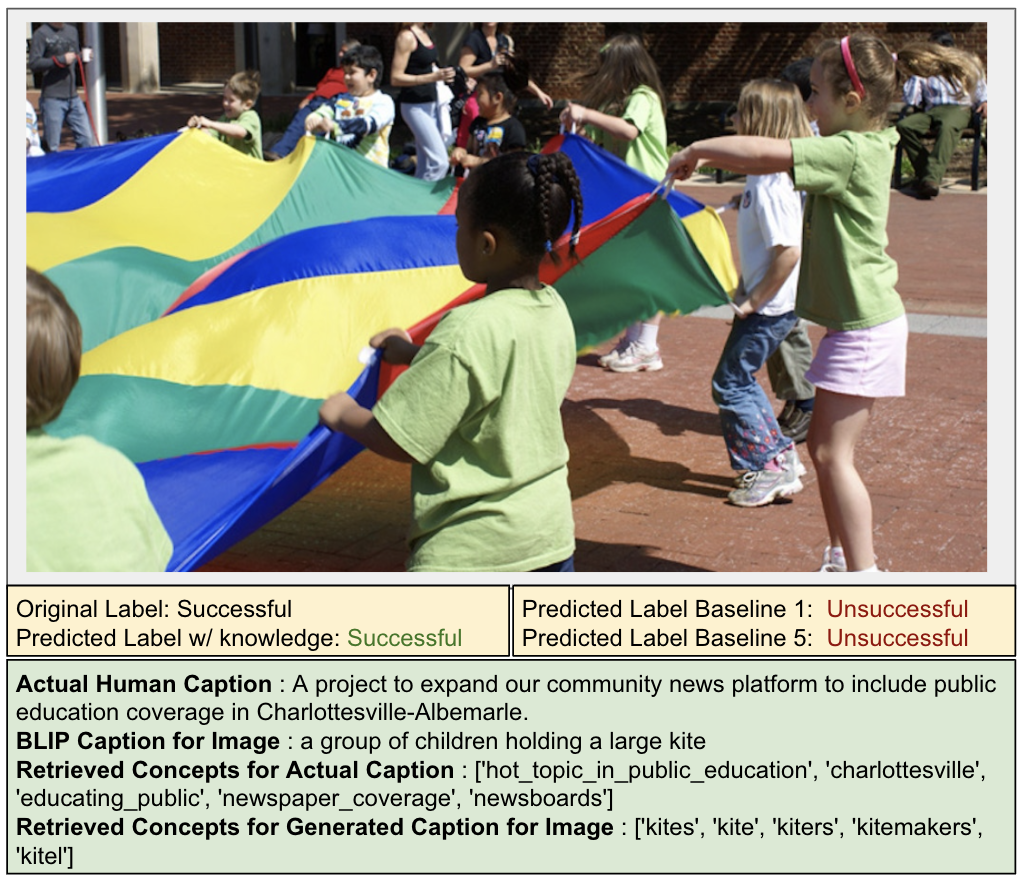
\includegraphics[width=8.5cm]{Figures/erroranalysis/error-analysis-sucess-community-project2.png}
\vspace{-2.2em}
\caption{The yellow box contains the model prediction with knowledge and two baseline models. The green box shows the actual caption, BLIP caption, and retrieved concepts for each modality.}
\vspace{-1em}
\label{fig:error-analysis-kites-educating-public}
\end{figure} 

% \vspace{-1em}
\subsection{Error Analysis}
\vspace{-1mm}
Overall, this analysis aims to explore the contribution of contextual congruence utilizing KGs in multimodal models, as well as limitations compared to baseline models. Hence, we examined a small number of data points where models with knowledge predicted correctly and incorrectly. We make the following observations:
%We delve into various scenarios where the improved model surpasses the baseline's shortcomings and identifies cases where the improved model falters due to the incorporation of noisy knowledge retrieval. By understanding these dynamics, we gain insights into the strengths and weaknesses of the enhanced model, contributing to a more nuanced understanding of its performance. Baseline models are the initial benchmark against which advancements are evaluated. However, in capturing the multimodal semantic relationships, these models display significant limitations, often struggling with complex patterns and nuanced relationships within the data. The improved model builds upon these weaknesses, incorporating commonsense knowledge from Conceptnet to overcome the baseline's shortcomings. While the improved model generally outperforms the baseline, its reliance on noisy knowledge retrieval presents its own set of challenges.

\noindent \textbf{Erroneous Omissions in Baseline Models.}  In Figure \ref{fig:error-analysis-kites-educating-public}, %it could be seen how 
the model with knowledge captures the important concepts or events that connect the image and text to prevent incorrect predictions, misclassifications, and an overall lack of precision. For instance, the baseline models can possibly recognize only objects and shallow details, while additional knowledge and relationships in between provide deeper context into the meaning of the content. The concept \textit{'hot\_topic\_in\_public\_education'} showcases students as \textit{‘kitemakers’}, \textit{'educating\_public'}  to support innovative teaching methods by \textit{'newspaper\_coverage'}. Such additional richer contextual knowledge helps the model to make better inferences for the meaning of content. 
%Consequently, the improved model excels in scenarios where the baseline faltered. It showcases better accuracy, improved generalization, and higher predictive power. Notably, these could be seen 
Similar limitations for baselines and advantages of knowledge infusion appear in  Figures \ref{fig:error-analysis-poetry-graffiti}, \ref{fig:error-analysis-woofer-error-analysis} and \ref{fig:error-analysis-sucess-poet}. 

%[Noisy Knowledge Retrieval and Its Impact:] 
\noindent \textbf{Erroneous Commissions in the Improved Models.}  The incorporation of noisy knowledge retrieval mechanisms into the improved model introduces a new set of challenges. In some cases, the model retrieves information that is either irrelevant or contradictory to the context.
%, leading to flawed predictions. 
This phenomenon is particularly prominent when the BLIP model fails to capture the main entities in the context of the image. 
%While the improved model demonstrates impressive performance, it is not immune to the issues introduced by noisy knowledge retrieval. Instances where the model fails due to such noise could be seen in 
(see Figure \ref{fig:error-analysis-failure-mens-mental-health}) where the campaign talks about how abuse and mental health issues suffered by men are often neglected.
%which can be seen in t
The campaign advertisement depicts men in a smaller size and women in a larger size, symbolizing the disproportionate attention given to men’s issues compared to women's. 
%By highlighting this disparity, but since 
As the knowledge retrieved for the image is from ConceptNet through the BLIP caption, many noisy concepts get infused, such as \textit{'front\_wall'}, \textit{'wall\_placement'}, \textit{'front\_walls'}, \textit{'recolor\_wall'}. %it is difficult to understand the context.
This analysis highlights the trade-off between performance enhancement through complex modeling and the susceptibility to noisy knowledge. While the recall improves at the expense of precision with knowledge-infused models, in the case of any misclassifications, the model may predict if a marketing campaign will be successful which may lead to possible financial loss.

\noindent \textbf{Social Impact.} Understanding (and thereby predicting) multimodal persuasiveness has extensive application. These are both benign, as in purchasing products or services, or malicious where prediction is a paramount tool for ensuring safety. In this regard, we note high recall (i.e., low false negatives) without reducing precision (i.e., low false positives), along with higher AUC, warranting further investigation for improvements in fairness using our approach. This distribution of error bears on detection efficiency of critical importance when the cost of error is high and detection requires manual follow-up. While we demonstrate such enhancement for effective multimodal marketing, a similar approach will be necessary for other context-sensitive social and behavioral problems including toxicity and extremism, among others. Further, there are still unknown implications of these AI-enabled technologies for individuals and communities, specifically, underrepresented groups in society. This work specifically provides potential avenues to address social biases, inadvertently encoded in large foundation models (e.g., LLMs, LVMs, VLMs) using a framework that incorporates external knowledge in learning, for future work.

%The insights gained from this analysis offer guidance for future model refinement and robust knowledge infusion techniques

%In conclusion, this error analysis sheds light on the contrasting performances of baseline and improved models within the context of preidcing the success of Multimodal marketing campaign, While the improved model exhibits superior predictive capabilities, it is crucial to remain mindful of the challenges posed by noisy knowledge retrieval. Through a balanced approach, the field can continue to make strides towards more accurate and robust models.



\begin{figure}
  \centering
  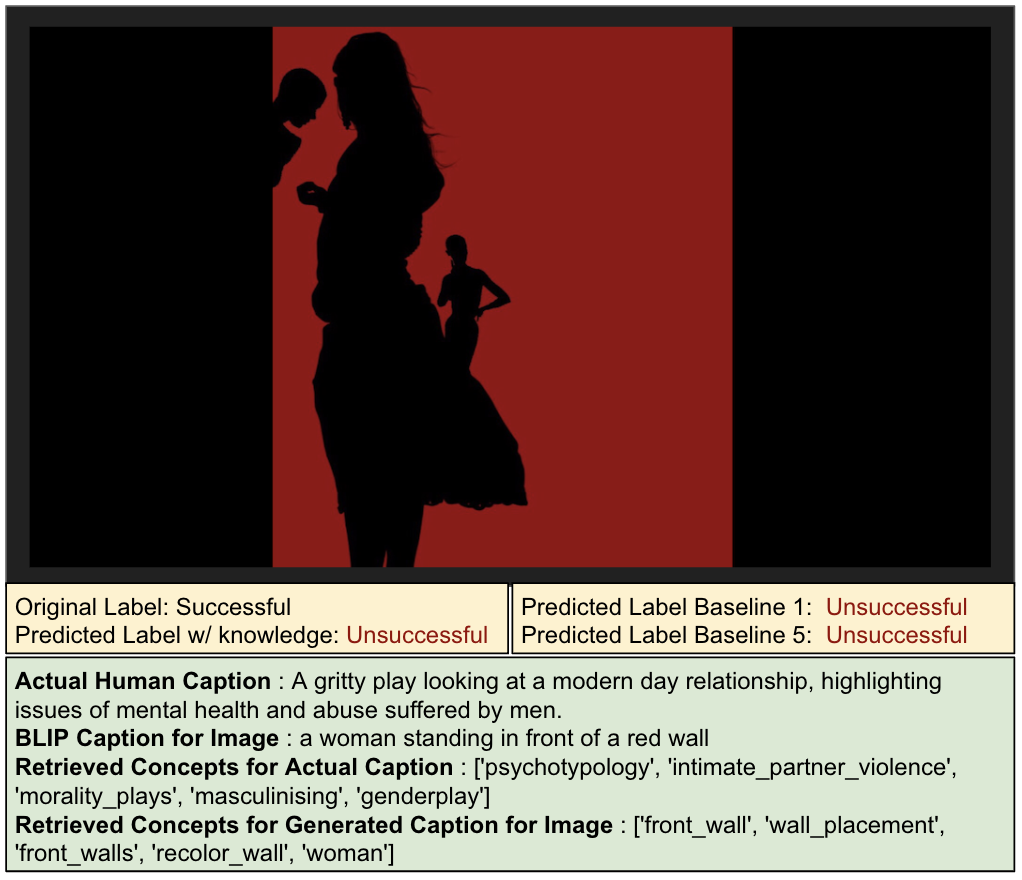
\includegraphics[width=8.5cm]{Figures/erroranalysis/error-analysis-failure-mens-mental-health2.png}
\vspace{-2.5em}
\caption{In this example, the model with knowledge could not also predicted accurate label along with other baseline models.}
% \textbf{Explanation:} The campaign talks about how abuse and mental health issues suffered by men are often neglected which can be seen in the campaign advertisement, which depicts men in a smaller size and women in a larger size, symbolizing the disproportionate attention given to women’s issues compared to men's. By highlighting this disparity, the campaign aims to raise awareness about the importance of addressing and supporting men's mental health struggles, ultimately advocating for equal treatment and resources for all genders.
% Since the knowledge retrieved for the image has lot of noisy concepts which get infused, such as 'front\_wall', 'wall\_placement', 'front\_walls', 'recolor\_wall', it is difficult to understand the context.}
\vspace{-2.5em}
\label{fig:error-analysis-failure-mens-mental-health}
\end{figure} 


\noindent \textbf{Limitations.} Utilizing KGs to improve contextual congruence across various modalities shows promise, particularly in crowdfunding marketing. While this approach can be adaptable to various fields, we acknowledge that further research is necessary to validate its effectiveness beyond crowdfunding. We also recognize that the knowledge-infused approach does encounter challenges with noisy triples from the KG, underscoring the need for enhanced robustness. We limited our experiments to the open-source smaller models due to the prohibitively high computational costs of larger models and left this for future research. While the approach is applied to crowdfunding, generally a benign domain, it can be misused with malicious intent such as creating highly persuasive and targeted misinformation campaigns. Therefore, we emphasize the need to follow ethical guidelines and responsible use of these novel approaches to prevent negative outcomes. The data used in this study may contain possible artifacts based on the "country" attribute, which we leave to address in future work. We anonymized our dataset to omit any identifiable information.  

% \section{Error Analysis}
% \label{sec:error-analysis}
% \input{7-ErrorAnalysis}


% \vspace{-1em} 
\section{Conclusion}
\label{sec:conclusion}
\vspace{-1mm}
Online multimodal marketing 
%is a human-centered process, which 
involves both image and text; hence, it provides an ideal domain for computing the relationship between these two modalities.  The domain also offers a success metric for the adequacy of a semantic interpretation; good interpretations are those that predict which image-text pairs will result in successful campaigns.
%requires an understanding of consumer behavior and perception. 
We developed a computational approach to capture the environmental context and congruence in multimodal online marketing content.
%that will enable more effective marketing materials and practices. 
External knowledge from KGs (e.g., ConceptNet)  enhanced the multimodal representation that %narrowed down 
decreased the semantic distance between the two modalities of a multimodal content, capturing the cross-modal semantic relationships better. External knowledge from KGs improved the 
%performance of a downstream task such as 
the success prediction of online crowdfunding campaigns. The approach facilitates the prediction of successful marketing campaigns, including the crowdfunding application studied here and more generally, the effectiveness of persuasive economic and public service campaigns.


% \begin{figure}[htb]
% % \centering
% \includegraphics[width=0.6\textwidth]{aaai2024/Figures/poetry-error-analysis.pdf}
% \caption{Comparison of Models}
% \label{fig:model-comparison}
% \end{figure}

% \vspace{-0.5em}
% \begin{figure}
%   \centering
%   \includegraphics[width=\linewidth]{aaai2024/Figures/poetry-error-analysis.png}
% \vspace{-1em}
% \caption{Pie chart showing type of Projects  and their percentages in Kickstarter \\ 
% % Model with knowledge & \quad \text{\Large\checkmark} \\
% % % \hline
% % Baseline Model 1 ( MMBT )  & \quad \text{\Large$\times$} \\
% % % \hline
% % Baseline Model 2 ( BLIP )  & \quad \text{\Large$\times$} \\
% \textbf{Actual Human Caption}: Looking to Publish a Third Poetry Volume with your help...\\
% \textbf{BLIP Caption for Image}: a book sitting on top of a wooden table \\
% \textbf{Retrieved Concepts for Actual Caption}: ['poetry\_book', 'book\_of\_poetry', 'poetry\_readings', 'poetry\_section', 'books\_poems'] \\
% \textbf{Retrieved Concepts for Generated Caption for Image}: ['book\_table', 'put\_book\_on\_shelf', 'book\_furniture', 'books\_on\_bookshelf', 'wooden\_table'] \\
% \textbf{Explanation}: The campaign image contains the cover of the ‘poetry\_book’ placed on the ‘wooden\_table’ or the ‘book\_table’. 
% \begin{center}
% \begin{tabular}{|c|c|}
% \hline
% \textbf{Model} & \textbf{Status} \\
% \hline
% Model with knowledge & \quad \text{\Large\checkmark} \\
% \hline
% Baseline Model 1 ( MMBT )  & \quad \text{\Large\checkmark} \\
% \hline
% Baseline Model 2 ( BLIP )  & \quad \text{\Large\checkmark} \\
% % \hline
% % Baseline Model Y & \adjustimage{width=1em,valign=m}{example-image-B}\quad \text{\Large$\times$} \\
% % \hline
% % Baseline Model Z & \adjustimage{width=1em,valign=m}{example-image-B}\quad \text{\Large$\times$} \\
% \hline
% \end{tabular}
% \end{center}
% }
% \vspace{-1em}
% \label{fig:example-image}
% \end{figure} 

% \begin{figure}
%   \centering
%   \includegraphics[width=\linewidth]{aaai2024/Figures/poetry-error-analysis.png}
  
%   \caption{Pie Chart: Distribution of Project Types and Percentages on Kickstarter}
%   \label{fig:project-distribution}
  
%   \vspace{1em}
  
%   \textbf{Actual Human Caption}: Looking to Publish a Third Poetry Volume with your help...

%   \textbf{BLIP Caption for Image}: A book sitting on top of a wooden table
  
%   \textbf{Retrieved Concepts for Actual Caption}: ['poetry\_book', 'book\_of\_poetry', 'poetry\_readings', 'poetry\_section', 'books\_poems']
  
%   \textbf{Retrieved Concepts for Generated Caption for Image}: ['book\_table', 'put\_book\_on\_shelf', 'book\_furniture', 'books\_on\_bookshelf', 'wooden\_table']
  
%   \textbf{Explanation}: The campaign image contains the cover of the ‘poetry\_book’ placed on the ‘wooden\_table’ or the ‘book\_table’. 
  
%   \begin{center}
%     \begin{tabular}{|c|c|}
%       \hline
%       \textbf{Model} & \textbf{Status} \\
%       \hline
%       Model with knowledge & \quad \text{\Large\checkmark} \\
%       \hline
%       Baseline Model 1 (MMBT) & \quad \text{\Large\checkmark} \\
%       \hline
%       Baseline Model 2 (BLIP) & \quad \text{\Large\checkmark} \\
%       \hline
%     \end{tabular}
%   \end{center}
% \end{figure}








% \begin{center}
% \begin{tabular}{|c|c|}
% \hline
% \textbf{Model} & \textbf{Status} \\
% \hline
% Model with knowledge & \quad \text{\Large\checkmark} \\
% \hline
% Baseline Model 1 ( MMBT )  & \quad \text{\Large\checkmark} \\
% \hline
% Baseline Model 2 ( BLIP )  & \quad \text{\Large\checkmark} \\
% % \hline
% % Baseline Model Y & \adjustimage{width=1em,valign=m}{example-image-B}\quad \text{\Large$\times$} \\
% % \hline
% % Baseline Model Z & \adjustimage{width=1em,valign=m}{example-image-B}\quad \text{\Large$\times$} \\
% \hline
% \end{tabular}
% \end{center}

% \clearpage
\newpage

% \begin{acks}
% To Robert, for the bagels and explaining CMYK and color spaces.
% \end{acks}

%% The next two lines define the bibliography style to be used, and
%% the bibliography file.
\bibliographystyle{ACM-Reference-Format}
\bibliography{references}

\clearpage

% \section{Paper Checklist}
% \label{sec:paper-checklist}
% \input{aaai2024/8-Checklist}
% \appendix

\clearpage

\section{Appendix}
\label{sec:otherappendix}
\subsection{Implicit and Explicit Context}
\label{sec:implicit-explicit-context}
Implicit context refers to the latent relationships and dependencies inferred by capturing the surrounding information environment through mechanisms, such as self-attention for transformers, gating for RNNs, and co-occurrence for Word2Vec. More specifically, the self-attention mechanism 
%allows the model to attend 
guides the model by assigning different weights to more relevant parts of the input sequence to capture dependencies between elements.
Explicit context refers to the information that is clearly stated in the content (e.g., text, image) without requiring additional interpretation or inference to understand. It is provided 
%explicitly provided 
alongside the input sequence to enhance its representation and understanding. Knowledge graphs and ontologies can be used to provide this contextual information as external knowledge. We utilize ConceptNet in this study, which provides external knowledge as a structured representation of real-world concepts and their relationships.


\subsection{Example data points with captions}
The following examples are from our dataset. Similar to the example in Section \ref{sec:intro} and Table \ref{tab:generated-caption-two-women}, we generated captions with and without knowledge for Figures \ref{fig:muslim-cap} and \ref{fig:ruler} and provided in Table \ref{tab:generated-captions}.  

\begin{figure}[hbt!]
  \centering
  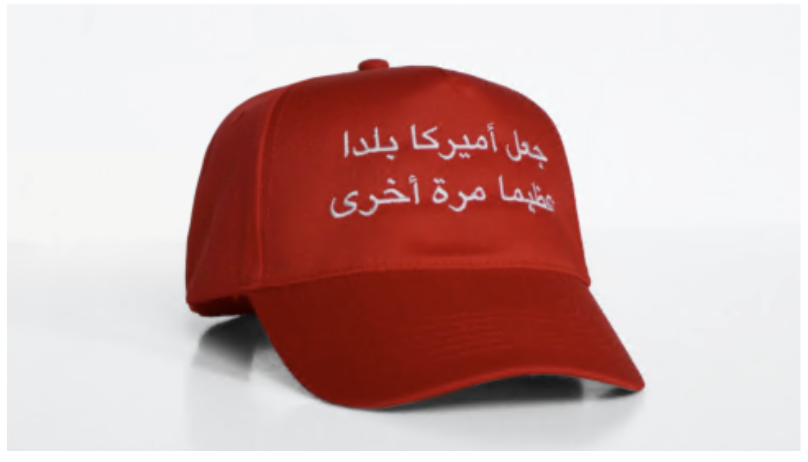
\includegraphics[width=8.5cm]{Figures/muslim_cap.png}
\vspace{-1em}
\caption{\textbf{Actual caption:} "Let's remind everyone that Muslim Americans are a part of our country and that they, too, make America great."}
% \vspace{-1.5em}
\label{fig:muslim-cap}
\end{figure} 

\begin{figure}[hbt!]
  \centering
  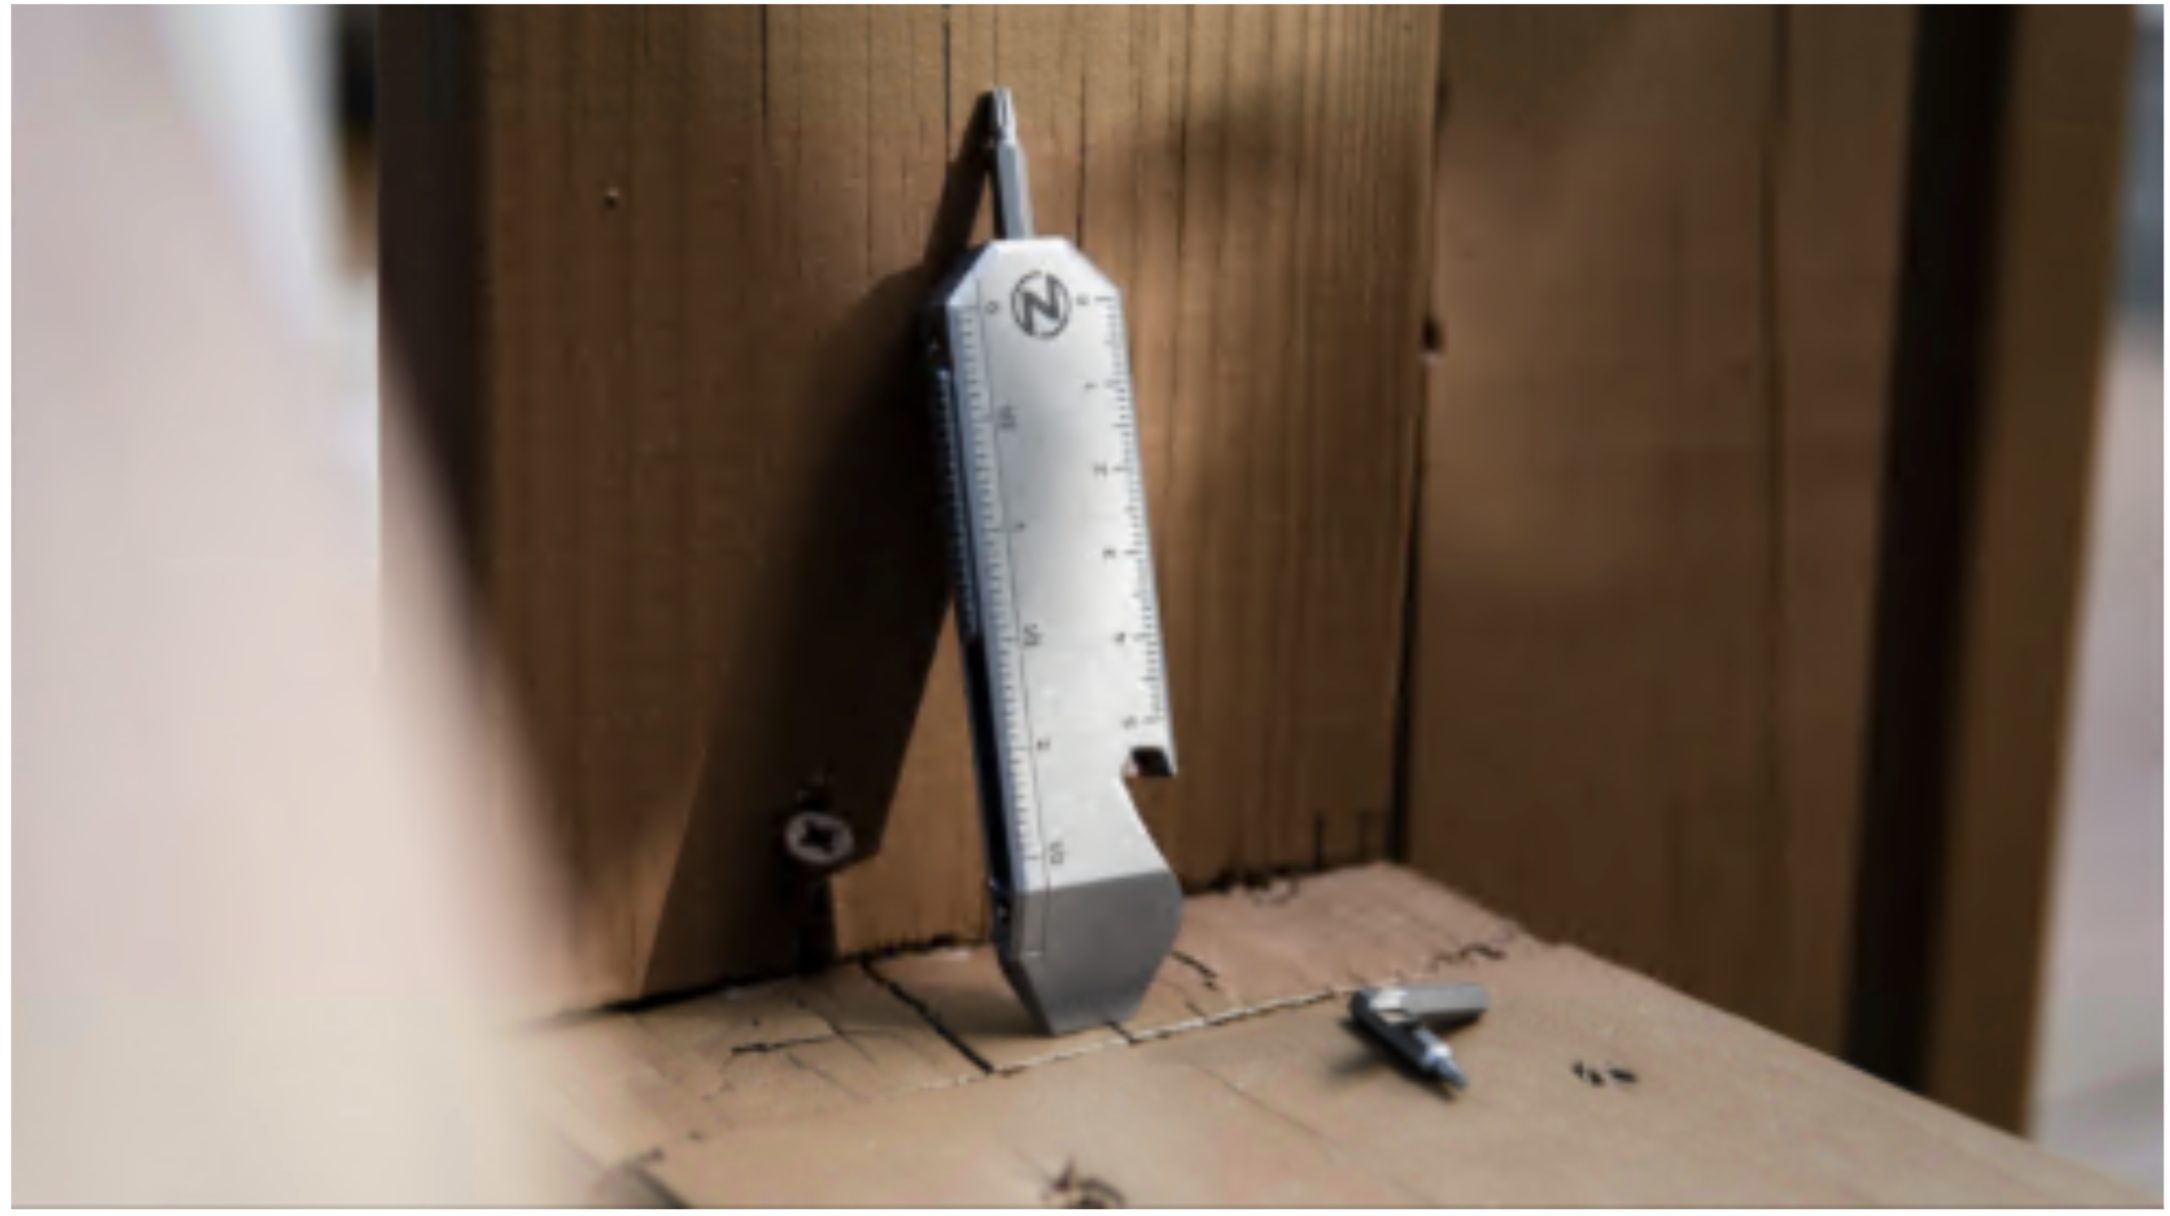
\includegraphics[width=8.5cm]{Figures/ruler.png}
% \vspace{-1em}
\caption{ \textbf{Actual caption:} " A TSA-compliant multi-tool with an innovative internal bit storage compartment"}
\vspace{-1.5em}
\label{fig:ruler}
\end{figure} 

\begin{table*}[!htbp]
  % \setlength\extrarowheight{-2pt}
  \centerline{%
    \begin{tabular}{p{1cm}p{2cm}p{10cm}p{1cm}}
    \toprule[3pt]
   \textbf{Model} & \textbf{Knowledge} & \textbf{Caption} & \textbf{Figure Label} \\
    \toprule[1pt]
    BLIP2 & No& a red baseball cap with arabic writing on it & \ref{fig:muslim-cap} \\
    \toprule[1pt]
    BLIP2 & Yes & muslim Americans are a part of our country and that they, too, make America great
    & \ref{fig:muslim-cap} \\ 
    \toprule[1pt]
    Llava & No & The image features a red cap with white lettering, likely a "Make America Great Again" hat, positioned on a white surface. The hat has Arabic writing on it, suggesting it is meant to convey a message of inclusivity and support for Muslim Americans. The message on the cap reads, "Muslim Americans also make America great." This serves as a reminder that Muslim Americans contribute significantly to the country and are essential in making America great, just like individuals from various backgrounds. & \ref{fig:muslim-cap} \\ 
    \toprule[1pt]
    Llava & Yes & The image features a red cap with white lettering, likely a "Make America Great Again" hat, placed on a white surface. The hat displays Arabic writing, which says, "Muslim Americans also make America great." This message emphasizes the importance of recognizing and appreciating the contributions of Muslim Americans to the nation, reminding people that they, too, play a vital role in making America great. The concept of Americanization refers to the process of adapting to American culture, values, and traditions, and this hat promotes the idea of Muslim Americans actively participating in and enriching the American society. & \ref{fig:muslim-cap} \\ 
    \toprule[3pt]
    BLIP2 & No &  a ruler is sitting on top of a piece of wood
    & \ref{fig:ruler} \\ 
    \toprule[1pt]
    BLIP2 & Yes &  a ruler is sitting on top of a piece of wood
    & \ref{fig:ruler} \\ 
    \toprule[1pt]
    Llava & No &  The image features a silver ruler with an internal bit storage compartment, placed against a brown wooden background. The ruler appears to be a TSA-compliant multi-tool, designed for both measuring and carrying small tools securely while in transit. The ruler's unique storage feature allows it to hold bits or other small objects, making it a practical and convenient tool for various purposes.
    & \ref{fig:ruler} \\ 
    \toprule[1pt]
    Llava & Yes & The image features a silver ruler with an internal bit storage compartment, designed for carrying and organizing small tools or bits securely. \textbf{This TSA-compliant multi-tool is particularly useful for transporting and organizing military equipment or cargo, as it can easily fit into the compartments of aircraft. The innovative internal storage compartment allows for efficient use of space, making it a very handy tool to carry and transport in unmanned transportation devices or the cargo hold of aircraft}
    & \ref{fig:ruler} \\ 
    \bottomrule[3pt]
    \end{tabular}%
  }
\caption{For the image and text pairs (see Figures \ref{fig:muslim-cap} and \ref{fig:ruler}), the captions generated by the models BLIP2 and Llava, when the models were prompted with the Image and Text with and without external Knowledge. The knowledge is extracted from ConceptNet as explained in section \ref{sec:explicit-knowledge} and appended to the prompt input to these models. While the generated captions with knowledge show less hallucinations and more grounding, we leave further investigation of those to the reader as they are not the focus of this study.}
\label{tab:generated-captions}
\end{table*}


\subsection{Extended Exploratory Analysis}[hbt!]
Similar to what we did in the exploratory analysis described in Section \ref{sec:exploratory}, we created clusters for text and image modalities, but in different sizes this time, to show that our observations did not change as shown in Figure \ref{fig:context_congruence_across_data_size}. The clusters get denser and the centroids get closer between them. 


\begin{figure*}
  \centering
  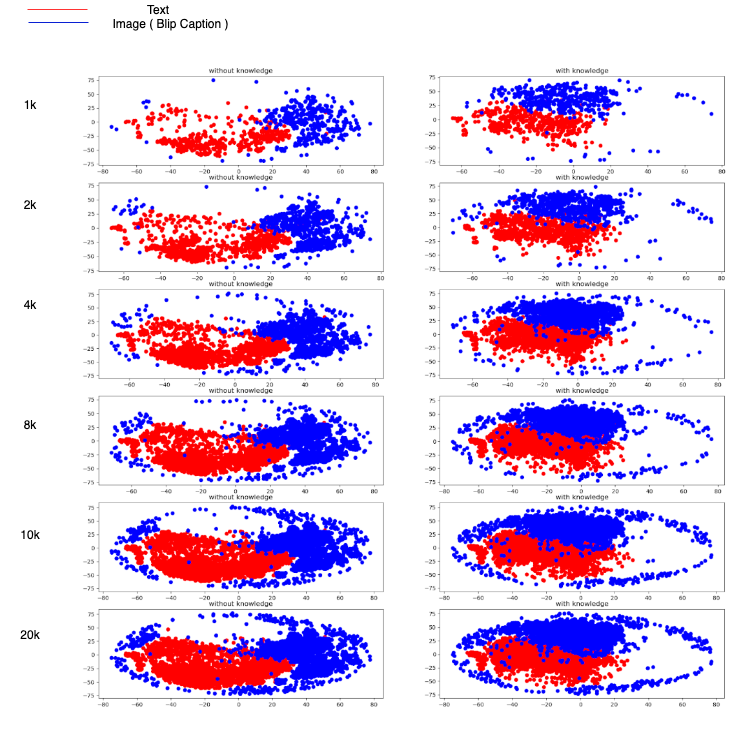
\includegraphics[width=18cm]{Figures/context_congruence_across_data_size.png}
% \vspace{-1em}
\caption{Cluster of the Embeddings of the BLIP Captions and the Marketing Caption Embeddings across varying data sizes. The gap between the image and text clusters reduces in the right plot with the addition of knowledge and can be seen across varying data sizes}
\vspace{-1.5em}
\label{fig:context_congruence_across_data_size}
\end{figure*} 


\subsection{Error Analysis Examples}
As we provided two examples for discussing different outcomes from our experiments including positive and negative, here we provide more examples for the reader to investigate further. The examples include Figures and their explanations
For Figure \ref{fig:error-analysis-woofer-error-analysis}, 
% \textbf{Explanation:} 
The campaign image promotes their 'subwoofer', 'dsp' solution by showing  ‘crowd\_concert’  of fans, their hands raised high in the air. It helps to convey the message  'many\_people\_to\_attend\_concert’.
For Figure \ref{fig:music-album-error-analysis}, 
% \textbf{Explanation:} 
The campaign ad is for a band which wants to promote its music by selling merchandise and by making  its digital copies and their merchandise available for purchase on their website. The band featured in the campaign ad wants to connect with their audience by providing specialized merchandise and releasing their music in digital formats. The noisy entities from the conceptnet ['bridge\_distance\_between\_people', 'bridge', 'bridges', 'bridgeness', 'holding\_up\_bridge']  fail to capture the important events in the pair of image and text.
For Figure \ref{fig:error-analysis-poetry-graffiti}, 
% \textbf{Explanation:} 
The campaign aims to showcase the intersection of 'performance\_poetry' by 'filmmaking'  by capturing these artistic expressions in unconventional locations such as  'graffiti' on  'front\_wall'.The campaign seeks to celebrate both the poet performers and the 'graffitists'.
For Figure \ref{fig:error-analysis-sucess-poet} 
% \textbf{Explanation:} 
Explanation : The campaign image showcases ‘poetry\_book’, ‘books\_of\_poems’, positioned over the ‘wooden\_table’ or the ‘book\_table’.
For Figure \ref{fig:error-analysis-failure-custom-windows}, 
% \textbf{Explanation:} 
The campaign ad is of a company named  “CUSTOMATIC”  which designs custom windows. lot of noisy concepts retrieved such as ‘word\_picture’ which get infused, may confuse the model.


% \vspace{-1.5em}
% \label{fig:custom-windows-error-analysis}
% \end{figure} 

\begin{figure}[htbp]
  \centering
  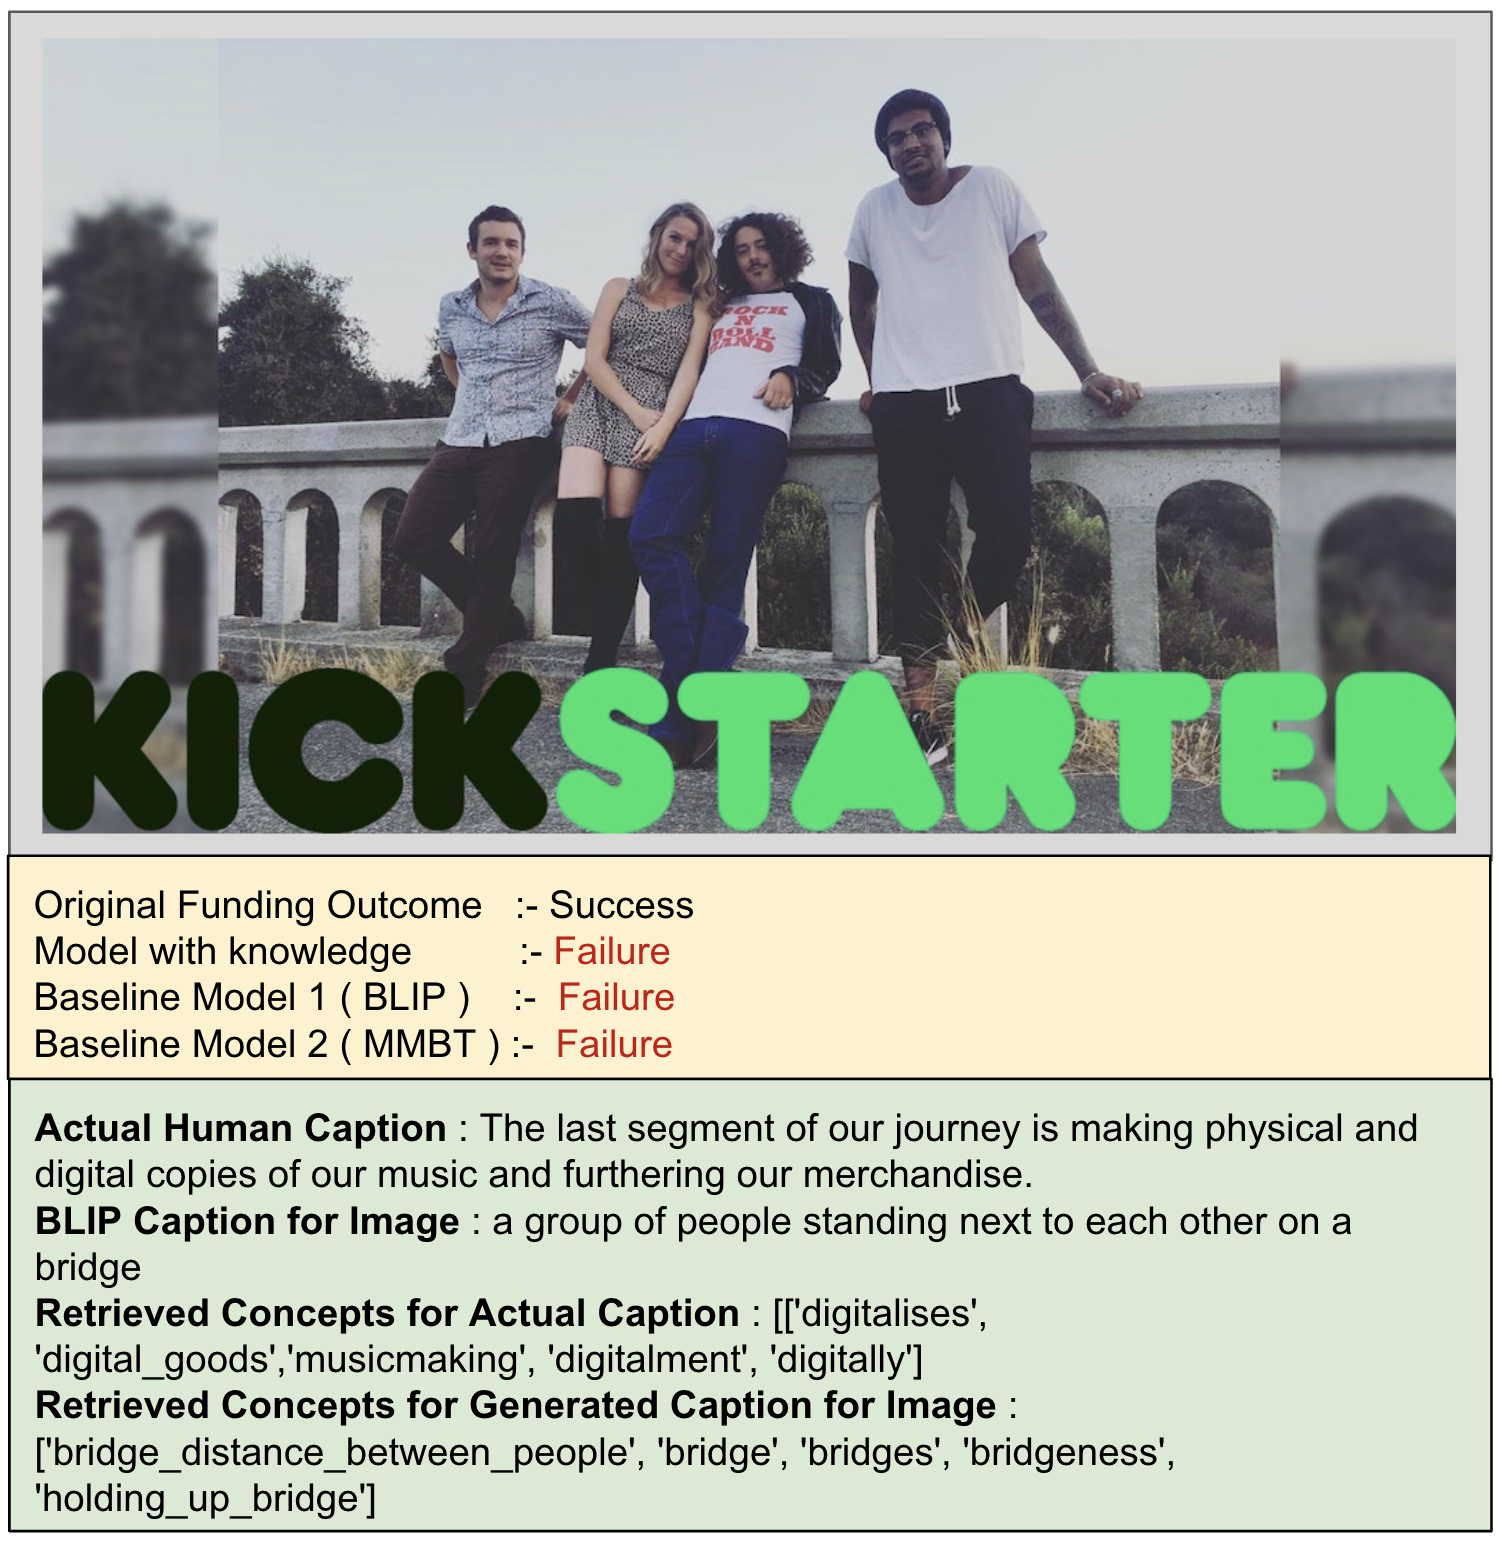
\includegraphics[width=8.5cm, height=8.5cm]{Figures/erroranalysis/error-analysis-music-band.png}
\vspace{-1em}
\caption{In the yellow box, the prediction of the model with knowledge, blip model and MMBT, In the green box, actual caption, blip caption, retrieved concepts for each modality.\\
}
\vspace{-1.5em}
\label{fig:music-album-error-analysis}
\end{figure}

\begin{figure}[htbp]
  \centering
  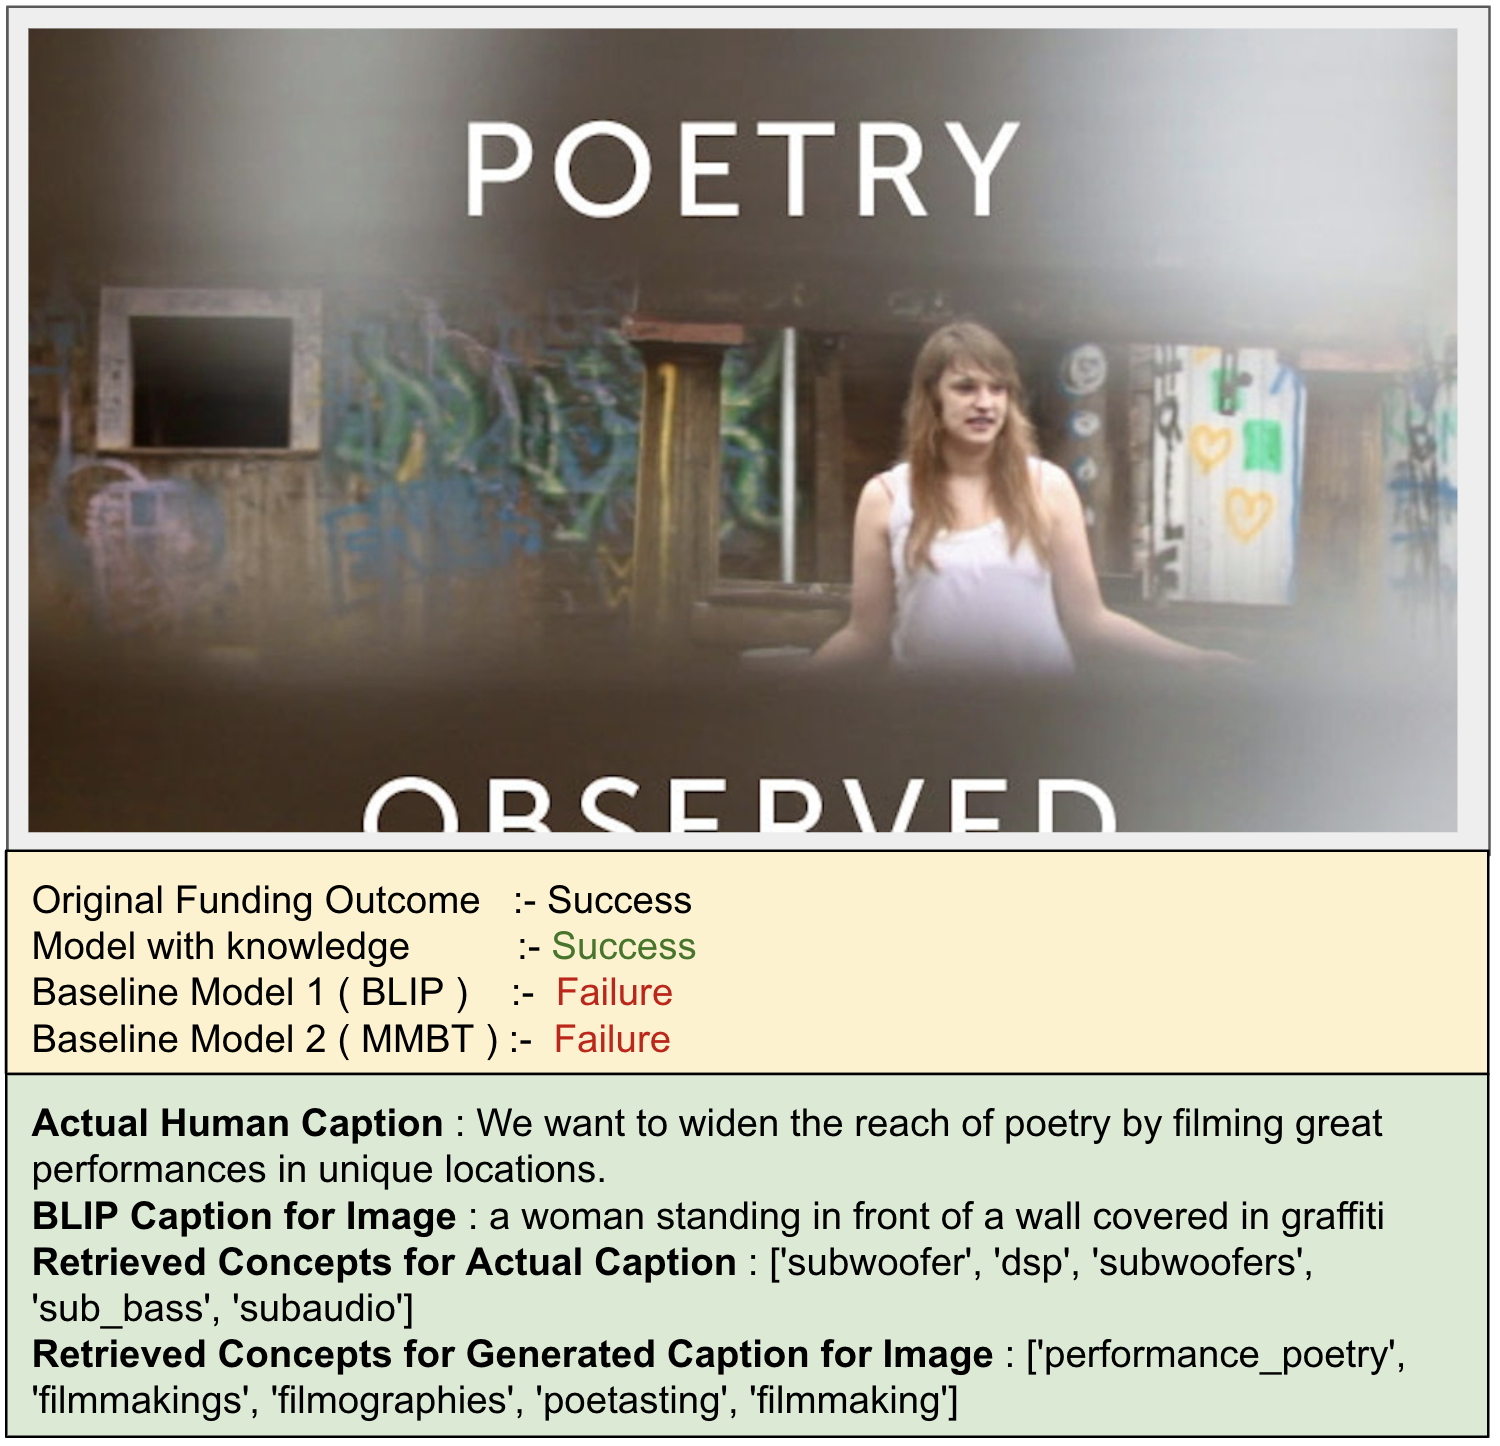
\includegraphics[width=8.5cm, height=8.5cm]{Figures/erroranalysis/error-analysis-sucess-poet-graffiti.png}
\vspace{-1em}
\caption{In the yellow box, the prediction of the model with knowledge, blip model and MMBT, In the green box, actual caption, blip caption, retrieved concepts for each modality.\\ 
}
\vspace{-1.5em}
\label{fig:error-analysis-poetry-graffiti}
\end{figure}

\begin{figure}[htbp]
  \centering
  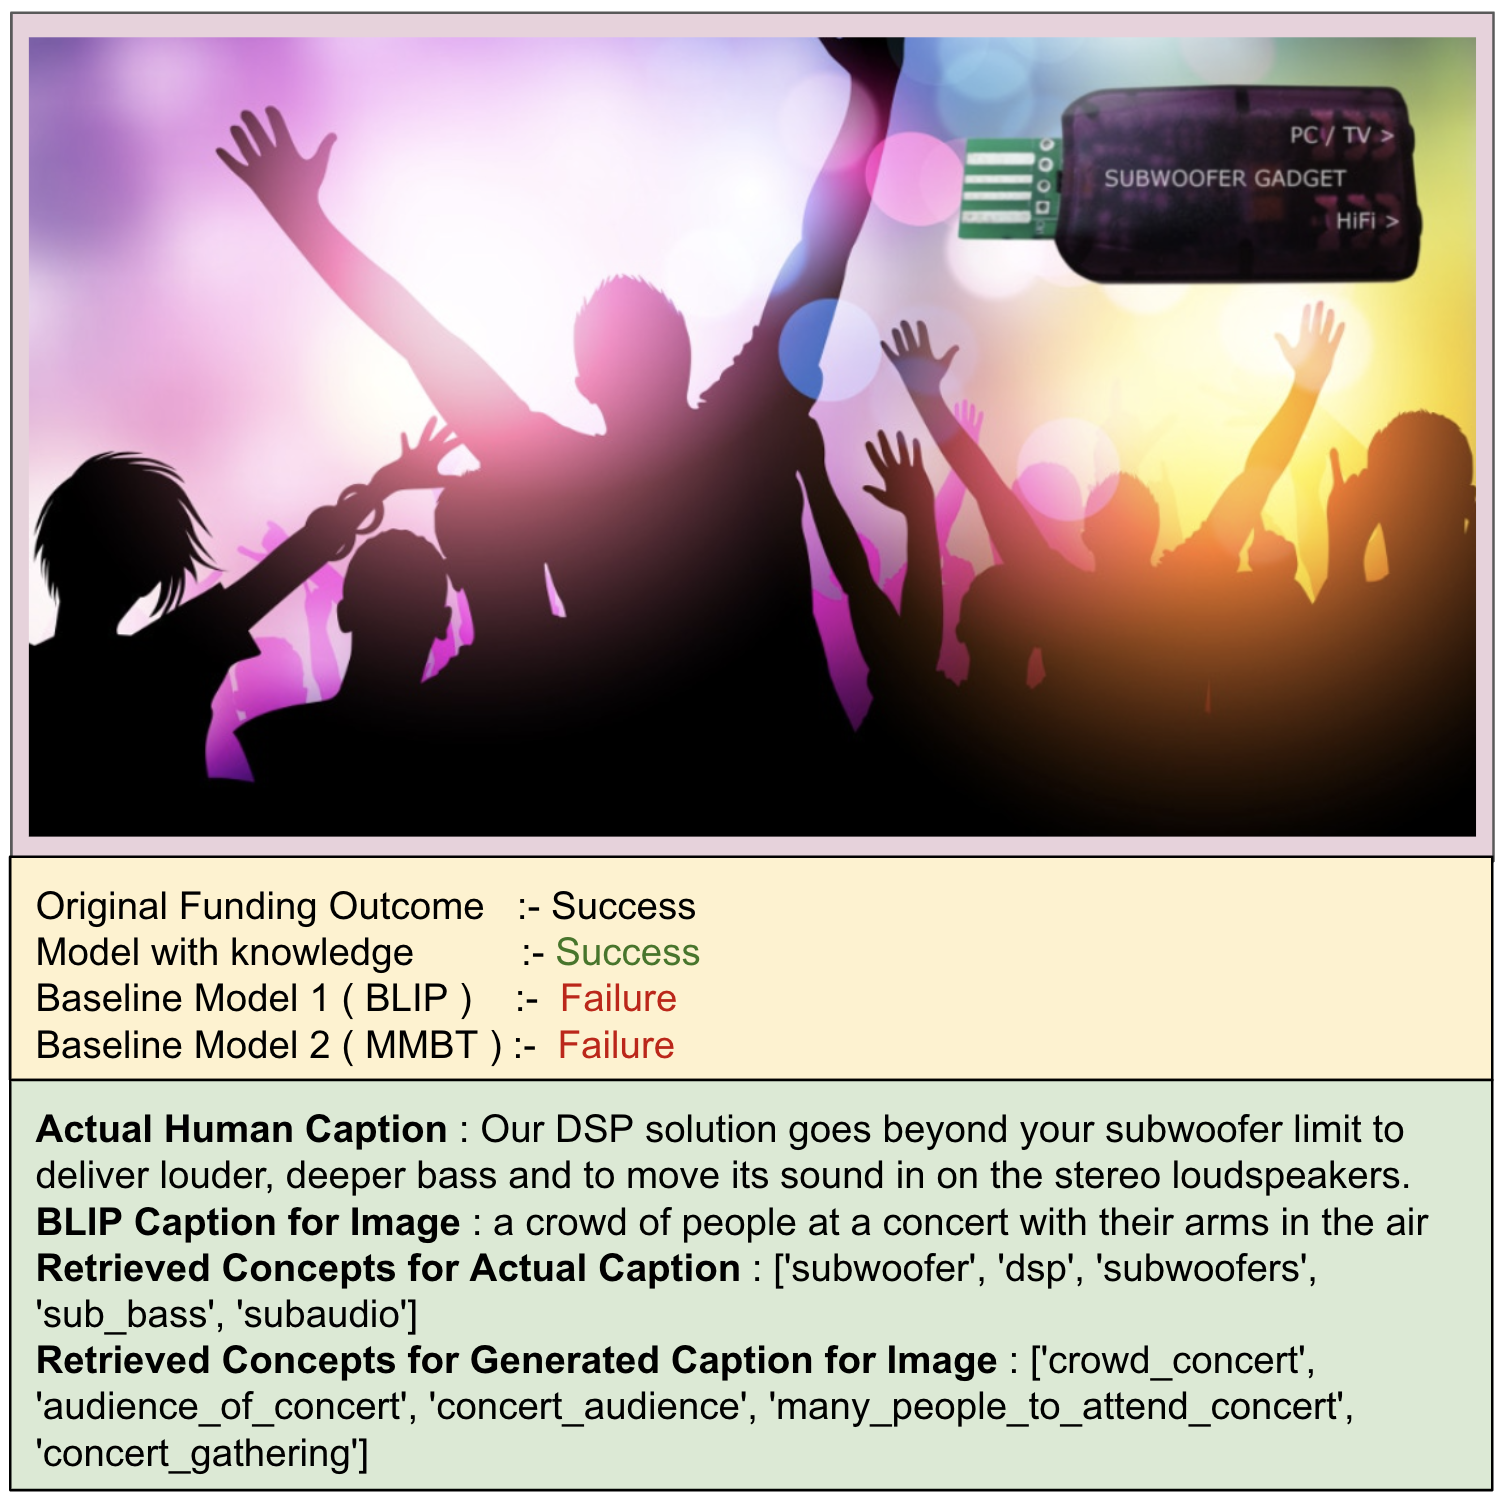
\includegraphics[width=8.5cm, height=8.5cm]{Figures/erroranalysis/error-analysis-sucess-woofer.png}
\vspace{-1em}
\caption{In the yellow box, the prediction of the model with knowledge, blip model and MMBT, In the green box, actual caption, blip caption, retrieved concepts for each modality.\\
% \textbf{Explanation:} The campaign image promotes their 'subwoofer', 'dsp' solution by showing  ‘crowd\_concert’  of fans, their hands raised high in the air. It helps to convey the message  'many\_people\_to\_attend\_concert’.
}
\vspace{-1.5em}
\label{fig:error-analysis-woofer-error-analysis}
\end{figure} 

\begin{figure}[htbp]
  \centering
  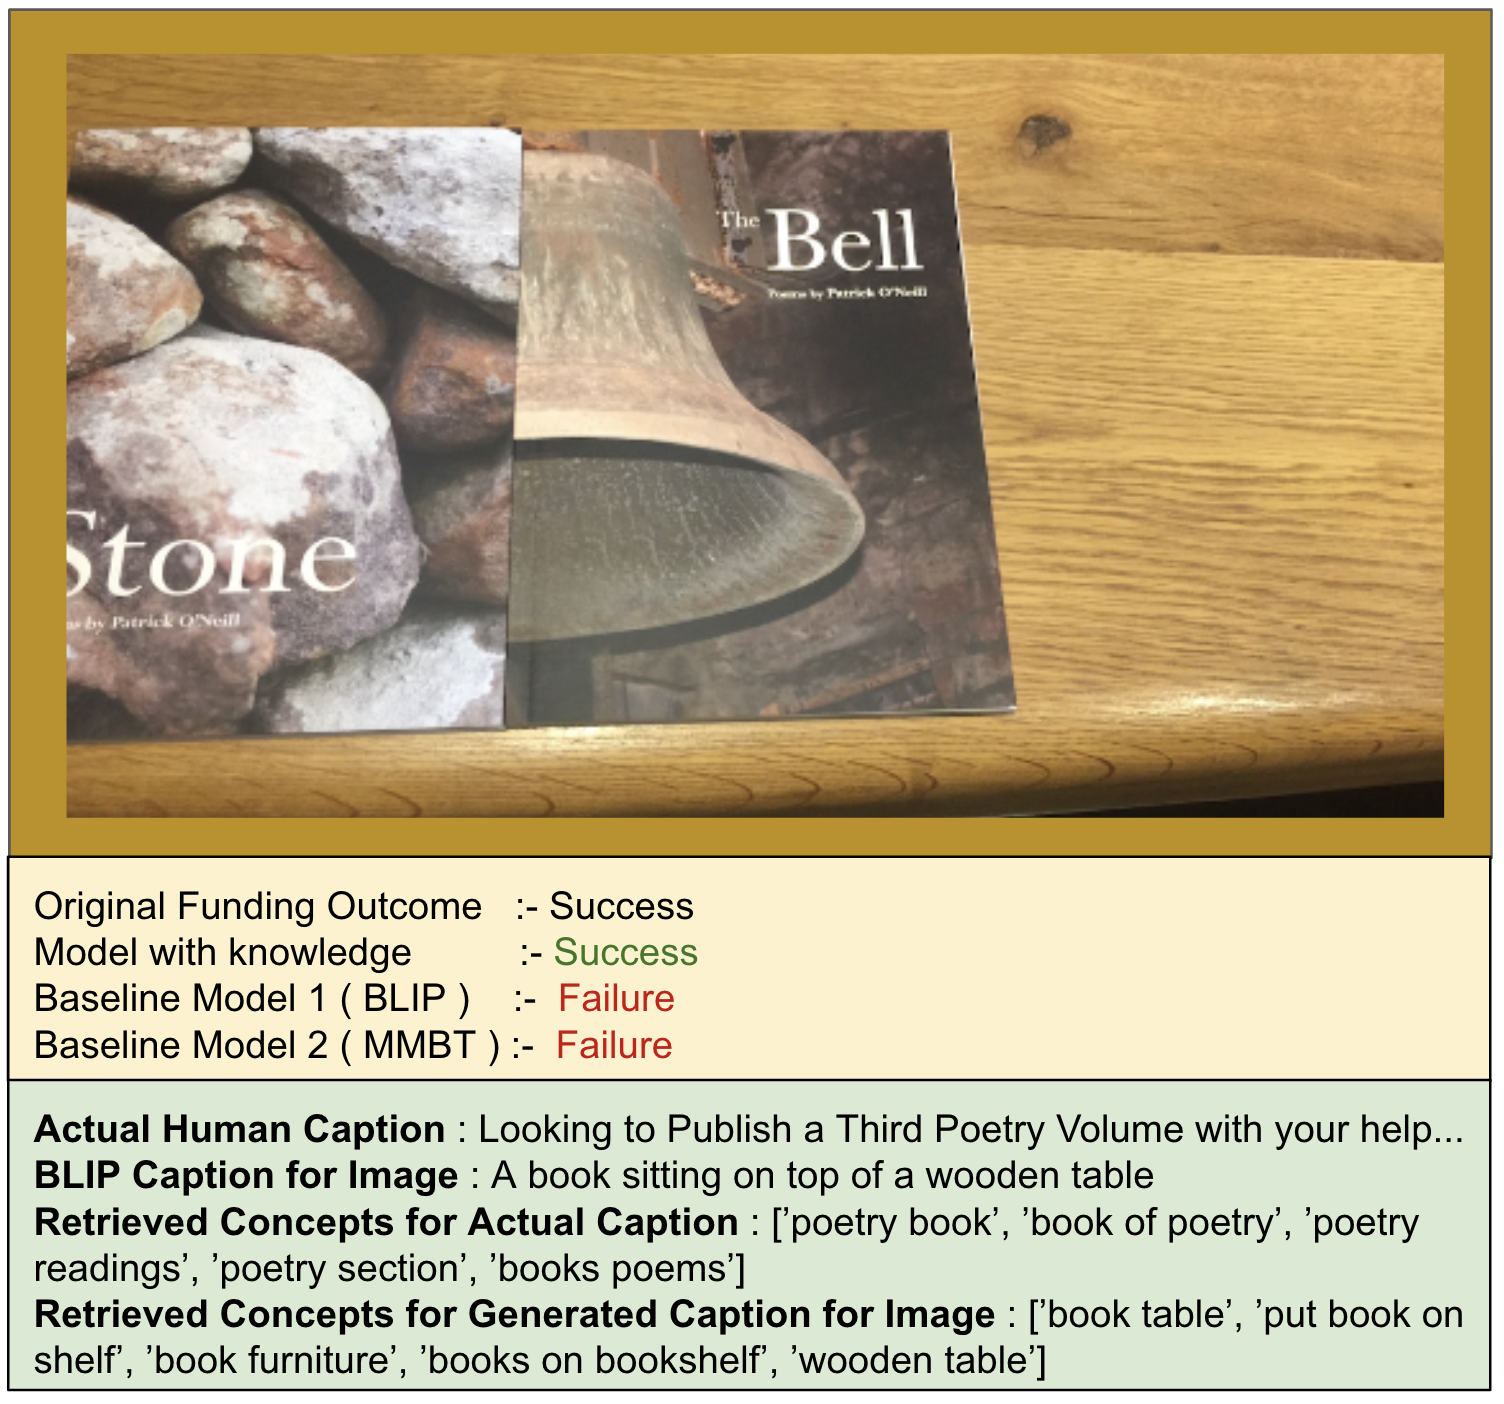
\includegraphics[width=8.5cm, height=8.5cm]{Figures/erroranalysis/error-analysis-sucess-poet.png}
\vspace{-1em}
\caption{In the yellow box, the prediction of the model with knowledge, blip model and MMBT, In the green box, actual caption, blip caption, retrieved concepts for each modality. \\
}
\vspace{-1.5em}
\label{fig:error-analysis-sucess-poet}
\end{figure} 

\begin{figure}[htbp]
  \centering
  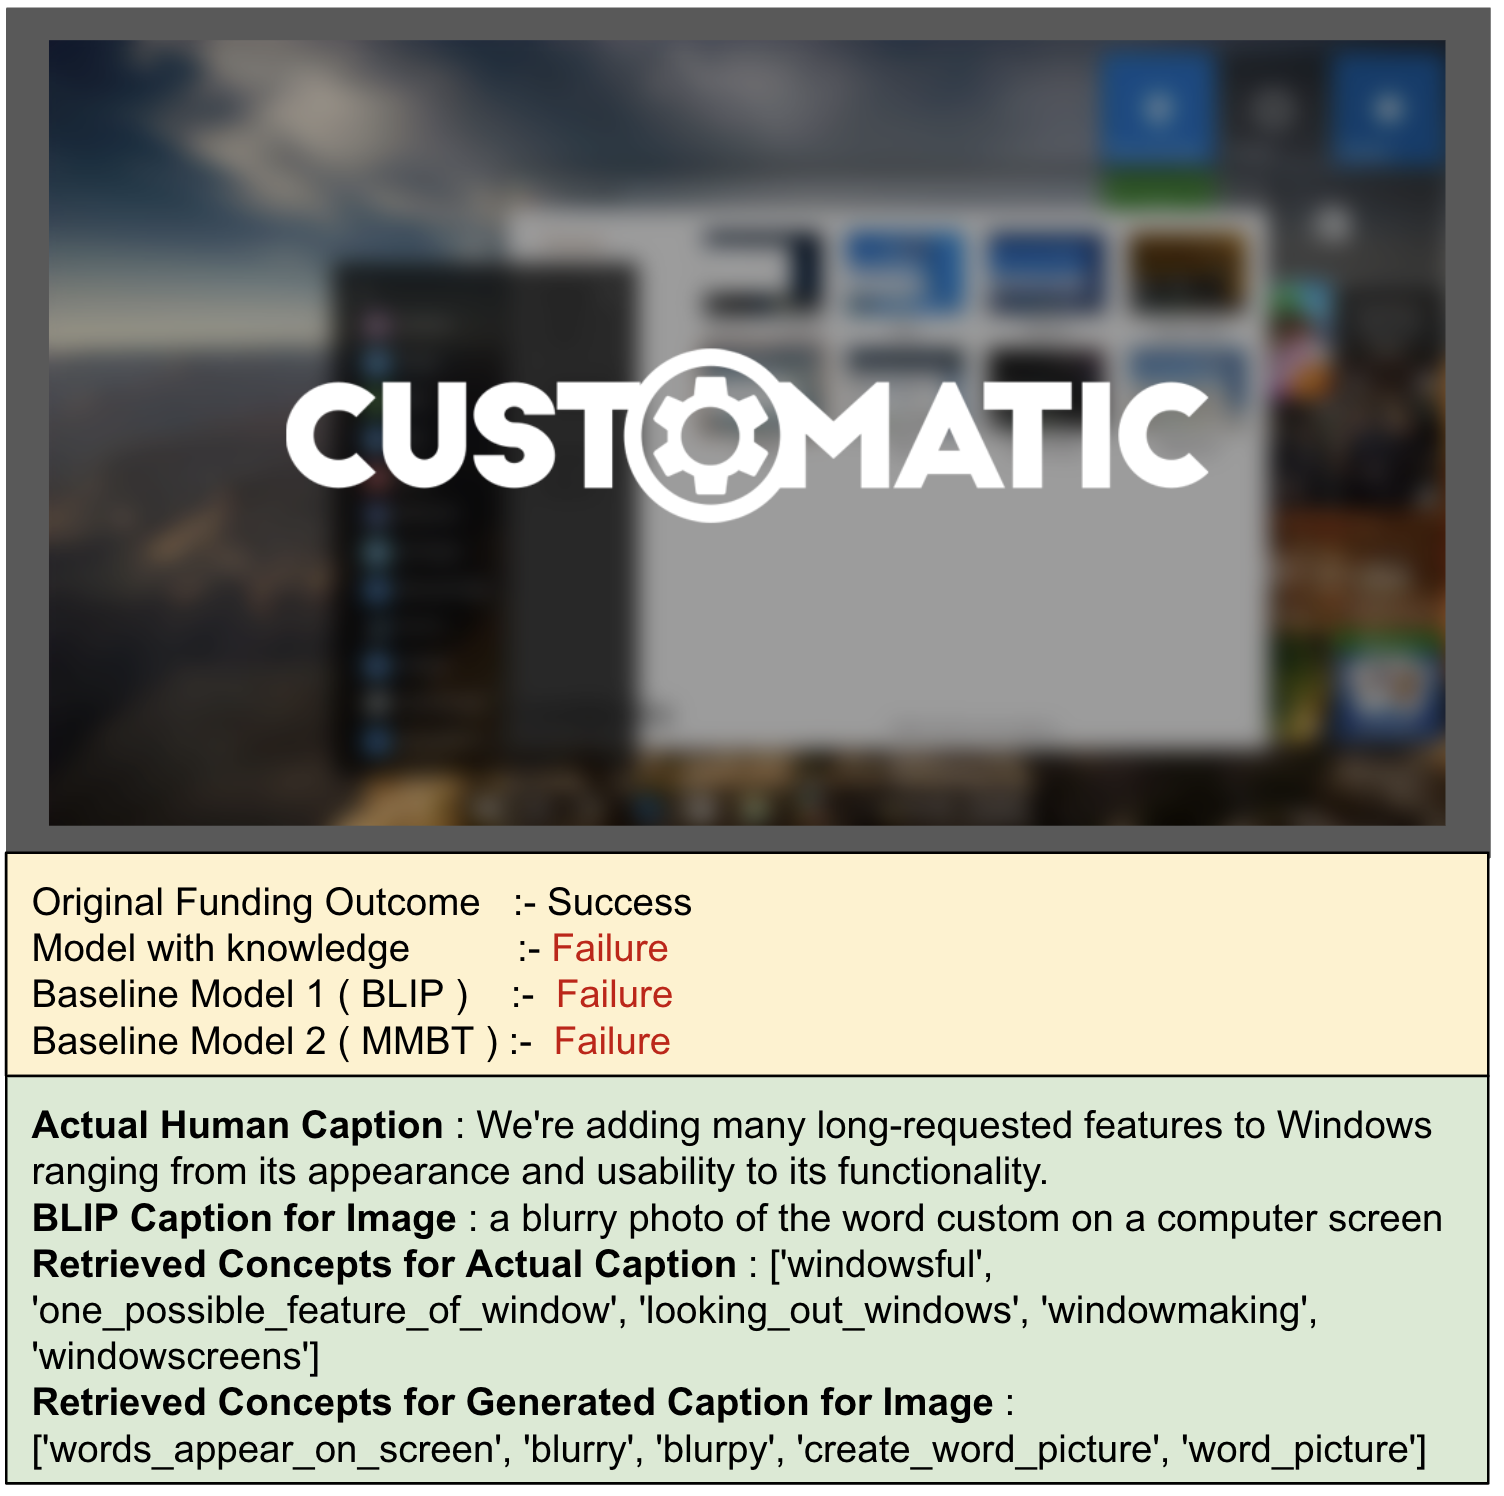
\includegraphics[width=8.5cm, height=8.5cm]{Figures/erroranalysis/error-analysis-failure-custom-windows.png}
\vspace{-1em}
\caption{In the yellow box, the prediction of the model with knowledge, blip model and MMBT, In the green box, actual caption, blip caption, retrieved concepts for each modality. \\
}
\vspace{-1.5em}
\label{fig:error-analysis-failure-custom-windows}
\end{figure}

\clearpage


\section{Data Appendix}
\label{sec:dataappendix}
\input{Dataapp}

\clearpage

% \section{Code Appendix}
% \label{sec:codeappendix}
% \input{Codeappendix}

\newpage


\end{document}
\endinput
%%
%% End of file `sample-sigconf.tex'.
